\documentclass[a4paper,14pt]{extreport}
\usepackage[utf8]{inputenc}


%Language&Font
%Geometry
\setcounter{secnumdepth}{4}
\setcounter{tocdepth}{3}
\usepackage[left=2cm,right=2cm,
    top=2cm,bottom=2cm,bindingoffset=0cm]{geometry}
\usepackage{breqn}
\linespread{1.3}
\usepackage[ukrainian]{babel}
%\setmainfont{Times New Roman}
%\usepackage{lmodern} 
\usepackage[T1]{fontenc}
\usepackage{layouts}
\usepackage{lipsum}


%========================================
%Table
\usepackage{booktabs, multirow} % for borders and merged ranges
\usepackage{soul}% for underlines
\usepackage[table]{xcolor} % for cell colors
\usepackage{changepage,threeparttable} % for wide tables

%========================================
%Math
\usepackage{mathtools}
\usepackage{float}
\usepackage{amsmath}
\newcommand{\angstrom}{\text{\normalfont\AA}}
%========================================
%Pictures
\usepackage{svg}
\usepackage{pgfplots}
\usepackage{graphicx}
\graphicspath{{img/}}
\DeclareGraphicsExtensions{.pdf,.png,.jpg,.eps, .svg, pgf}
\usepackage{caption}
\usepackage{subcaption}
\usepackage{hyperref}
\DeclareCaptionType{constrains}[Список][Список]

%========================================
%Титулка
%\title{Дипломна робота}
%\author{Носенко Артем Олексійович}
%\date{December 2021}


%========================================
%Table contents
\bibliographystyle{ieeetr}
\usepackage{hyperref}
\hypersetup{
    colorlinks,
    citecolor=black,
    filecolor=black,
    linkcolor=black,
    urlcolor=black
}

%========================================
%Body
\begin{document}
%\begin{titlepage}
%  \renewcommand\baselinestretch{0.75}\normalsize
%  \renewcommand\baselinestretch{1.25}\normalsize
 \begin{center}
Національна академія наук України \\
Міністерство освіти і науки України
  \vspace{0.25cm}
  
  \textbf{Державна наукова установа \\ 
  «Київський академічний університет»}
  \vspace{0.5cm}
  
  Кафедра прикладної фізики та наноматеріалів
  \\ Спеціальність 105 Прикладна фізика та наноматеріали
  
  \vspace{1cm}
  
  \large\textbf{МАГІСТЕРСЬКА  ДИПЛОМНА  РОБОТА} \\
  студента  \textbf{Носенка Артема Олексійовича}
 \end{center}
\begin{center}
 {На тему \large\textbf{«Моделювання електронної структури Ван-дер-Ваальсових матеріалів в межах ТФГ»}\par}
\end{center}
\vspace{0.5cm}

\hfill\parbox{12cm}{
\begin{flushleft}
 \hfill Науковий керівник: доктор фіз.-мат. наук, професор \\
 \hfill \underline{\hspace{4cm}} \hspace{1cm} Карбівський В. Л. \\
 \hfill Рецензент: доктор фіз.-мат. наук, професор \\
 \hfill \underline{\hspace{4cm}} \hspace{2cm} Хижун О. Ю. \\
\end{flushleft}}

\hfill\parbox{10cm}{
\begin{flushleft}
 \begin{center}
 \small
     \textbf{Робота допущена до захисту в ЕК} \\
     Завідувач кафедри \\
     доктор фіз.-мат. наук, професор \\
     \hfill \underline{\hspace{4cm}} \hspace{1cm} Лень Є. Г.  
 \end{center}
\end{flushleft}}

\hfill\parbox{10cm}{
\begin{flushleft}
 \begin{center}
 \small
     Засвідчую, що у цій магістерській роботі немає 
     запозичень з праць інших авторів без відповідних посилань \\
     Студент \underline{\hspace{4cm}} Носенко А. О.
 \end{center}
\end{flushleft}}

\vfill

\begin{center}
 Київ -- 2022
\end{center}
\end{titlepage}
\tableofcontents
\begin{center}
{\large \textbf{АНОТАЦІЯ}}
\end{center}

\textbf{Носенко А. О.} Моделювання електронної структури Ван-дер-Ваальсових матеріалів в межах DFT. \\
Кваліфікаційна робота магістра за спеціальністю 105 Прикдна фізика і наноматеріали, освітня програма Пркикладна фізика і наноматеріали. 
"--- Державна наукова установа «Київський академічний університет», кафедра прикладної фізики та наноматеріалів. "--- Київ "--- 2022.

З використанням підходів PBE GGA та SCAN meta-GGA, в рамках теорії функціоналу густини, було визначено параметри електронних властивостей 1T-TiX$_2$ (X = S, Se, Te). Зокрема, визначено оптимальний Хаббардовський параметр для досліджуваних сполук. Встановлена електронна природа 1T-TiS$_2$, 1T-TiSe$_2$, 1T-TiTe$_2$ та розрахована ширина забороненої зони для 1T-TiS$_2$.  

\textbf{Науковий керівник}: д.ф.-м.н. Карбівський В. Л.

\textbf{Елементи оформлення}: 13 рисунків, 4 таблиць, 1 список.

\textbf{Ключові слова}: діхалькогеніди перехідних металів, зонні розрахунки, теорія функціонала густини.



\bigskip

\clearpage

\thispagestyle{empty}
\begin{center}
{\large \textbf{SUMMARY}}
\end{center}

\textbf{Nosenko A. O.} Modeling of the electronic structure of van der Waals materials by means DFT. \\
Masters qualification work in specialty 105 Applied physics and nanomaterials, educational program Applied physics and nanomaterials "--- State Research Institution «Kyiv Academic University», Department of Applied physics and nanomaterials. "--- Kyiv "--- 2022.

Using the PBE GGA and SCAN meta-GGA approaches, the parameters of the electronic properties of 1T-TiX$_2$ (X = s, Se, Te) were determined within the framework of the density functional theory. In particular, the optimal Hubbard's parameter for the studied compounds was determined. The electronic nature of 1T-TiS$_2$, 1T-TiSe$_2$, 1T-TiTe$_2$ is established and the width of the band gap for 1T-TiS$_2$ is calculated.

\textbf{Research supervisor}: Doctor of Physical and Mathematical Sciences, \\ Karbivsky V. L.

\textbf{Design elements}: 13 Figures, 4 Tables, 1 list.

\textbf{Key words}: transition metal dichalcogenides, band calculations, density functional theory.




\chapter{Літературній огляд досліджуваних систем}
\section{Експериментальне та теоретичне дослідження електронної будови TiS2}
Після відкриття А. Геймом та К. Новосьоловим графену у 2004 році~\cite{Graphene}, знову зріс інтерес до двохвимірних матеріалів, зокрема до дихалькогенідів перехідних металів та їх інтеркаляційних сполук, які дуже сильно досліджувались у 80-х роках. Ці сполуки мають формулу MX$_{2}$ (X = S, Se, Te; M = Ti, Zr, Hf, V, Nb, Ta, Mo, W).

Дослідження електронної будови TiS$_{2}$ дали суперечливі висновки. З одного боку деякі розрахунки зонної структури приводять до непрямого перекриття p/d смуг між точками $\Gamma$ та $L$ в діапазоні від 0.2 до 1,5 еВ. Інші стверджують, що TiS$_{2}$ є вузько-щілинним напівпровідником. Експериментальні данні отримані за допомогою фотоемісії вказують на те, що поведінка даної сполуки схожа на напівпровідникову~\cite{semiconducter} або ж напівметалічну~\cite{semimetal}. Як відомо, TiS$_{2}$ має високу електронну провідність без зовнішнього легування, однак походження цієї високої провідності, будь то напівметал або сильно легований напівпровідник, обговорюється протягом декількох десятиліть, але деякі недавні GW, DFT розрахунки в поєднані з сканувальною зондовою мікроскопією, все ж таки, стверджують, що висока провідність обумовлена сильним самолікуванням~\cite{semimetal_or_semiconducter}. 

Щодо прикладного застосування, то даний матеріал успішно використовується у літій-іонних акумуляторах у якості катода. Коефіцієнт дифузії літію у TiS$_2$ порядку $10^{-8}-10^{-7}$ см$^2$/с, на один --- два порядки вище, ніж у широко використовуваних оксидних катодів. Недавні досліди показують, що комірки TiS$_2$ могуть зберігати більш ніж 50 \% початкової ємності після 35 років зберігання. Однією з важливих причин, чому TiS$_2$ був обраний як катодний матеріал для літій-іонних батарей, є те, що він має високу внутрішню електропровідність без зовнішнього легування. Це відрізняється від деяких інших популярних катодів таких, як LiFePO$_4$, для яких низька провідність була головною проблемою.

У 2003 році метод низькотемпературного газофазного синтезу(TiCl$_4$ + 2H$_2$S $\rightarrow$ TiS$_2$ + 4HCl), був успішно використаний для отримання нанотрубок на основі TiS$_2$~\cite{nanotube}. Аналіз їх морфології і структури показав, що трубки складаються з співвісних шарів сульфіду титану (відстань між шарами становить 0,57 нм) з атомним співвідношенням Ti:S =1:2, мають відкриті кінці, середні значення зовнішнього і внутрішнього діаметрів трубок складають ~20 - 30 і ~10 нм відповідно. У роботах~\cite{nanotube2,nanotube3} були вивчені процеси інтеркалювання нанотрубок TiS$_2$ літієм і воднем і обговорені можливості їх використання в якості матеріалів для водневих акумуляторів. Матеріалознавчі перспективи різних класів наноструктур багато в чому визначаються їх електронними властивостями, які можуть істотно відрізнятися від відповідних кристалічних (3D) фаз. Зазначені властивості в свою чергу залежать від атомної будови і геометрії наноструктур. Так, нанотрубки дисульфідів Mo, W є напівпровідниками, причому в залежності від діаметра і атомної конфігурації стінок (так званої хіральності) величина забороненої щілини різко змінюється. Навпаки, всі NbS$_2$-нанотрубки за своїми провідними властивостями є металами~\cite{nanotube4,nanotube5,nanotube6}.
\chapter{Density Functional Theory}
Шляхом публікації двох статей Хохенбергом та Коном у 1964 році~\cite{Hohenberg&Khon}, а також Коном і Шамом в 1965 році~\cite{Khon&Sham}, теорія електронної будови вийшла на зовсім новий рівень. Мабуть, найважливішим є те, що ТФГ це теорія взаємодіючої та корельованої системи електронів. Версія ТФГ Кона-Шама використовує метод незалежних частинок; вона будує допоміжну систему, яка визначає точно електронну щільність та енергію фактично взаємодіючої системи.

В ТФГ Кона-Шама всі обмінні та кореляційні ефекти включені в обмінно-кореляційний функціонал $E_{xc}[n]$, котрий залежить від густини $n(\textbf{r})$ електронів. 

\section{Підхід Кона-Шама}
Функціонал повної енергії може бути записаний, як~\cite{K-S energy}:
\begin{eqnarray}
 E[\psi_i] = 2\sum\limits_{i}\int\psi_i\left({{\hbar^2}\over{2m}}\right)\nabla^2\psi_id^3\textbf{r}+\int V_{ion}(\textbf{r})n(\textbf{r})d^3\textbf{r}+\nonumber \\
 {{e^2}\over{2}}\int {{n(\textbf{r})n(\textbf{r})}\over{|\textbf{r}-\textbf{r}^\prime|}}d^3\textbf{r}d^3\textbf{r}^\prime+E_{xc}[n(\textbf{r}^\prime)]+E_{ion}(R_i)
\end{eqnarray}

Де $V_{ion}$ -- повний електрон-іонний потенціал, $E_{xc}[n(\textbf{r}^\prime)]$ -- обмінно-кореляційний функціонал, $E_{ion}$ -- кулонівська енергія, $n(\textbf{r})$ -- електронна густина

\subsection{Теореми Кона-Шама}

\textbf{Перша теорема} говорить про те, що електронна щільність єдиним чином визначає оператор Гамільтона і, отже, всі характеристики системи.
Не можуть існувати два різні зовнішні потенціали, що призводять до однієї і тієї ж електронної щільності основного стану системи, іншими словами, електронна щільність основного стану однозначно визначається зовнішнім потенціалом.
Знаючи потенціал, ми знаємо Гамільтоніан системи, відповідно можемо знайти хвильову функцію системи та всі властивості системи, що визначаються електронною щільністю основного стану. Перша теорема показує зв'язок між зовнішнім потенціалом та електронною щільністю основного стану.

\textbf{Друга теорема} функціонал енергії, що визначає енергію квантового стану системи, визначає мінімальну енергію тоді і тільки тоді, коли електронна густина, що входить у функціонал, є реальною густиною основного квантового стану.
Таким чином, для знаходження точної енергії основного стану та його щільності, достатньо знати функціонал $E[n]$. Висновки цих теорем призводять до того, що для будь-якого зовнішнього потенціалу завжди можна знайти електронну густину та енергію основного стану, мінімізуючи цей функціонал.


\subsection{Самоузгоджене рівняння Кона-Шама}
Електронна щільність системи може бути знайдена з рішення самоузгодженого рівняння Кона-Шама, це випливає з наведених раніше теорем, яке можна записати так:

\begin{equation}
    \left[{{-\hbar^2}\over{2m}}\nabla^2+V_{ion}(\textbf{r})+V_H(\textbf{r})+V_{XC}(\textbf{r})\right]\psi_i(\textbf{r}) = e_i\psi_i(\textbf{r})
\end{equation}

Де $\psi_i$ -- хвильова функція стану $i$, $e_i$ -- власні значення, $V_H$ -- потенціал Хартирі, який відповідає за електронно-електронне відштовхування.

Явний вид обмінно-кореляційного потенціалу $V_{XC}$ ми не можемо знати принципово, тому його задають формально, функціональною похідною: 

\begin{equation}
    V_{XC} = \frac{\partial E_{XC}[n(\textbf{r})]}{\partial n(\textbf{r})}
\end{equation}

Для визначення об'ємно-кореляційного потенціалу використовують ряд наближень, про які ми поговоримо у наступному розділі.


\section{Методи апроксимації \textbf{$E_{xc}$}}
\subsection{LDA}
LDA (local density approximation) -- це клас наближень для обмінно-кореляційної енергії $E_{XC}$ у ТФГ, яка залежить виключно від електронної густини в кожній точці простору. Найуспішнішими локальними наближеннями є ті, що були отримані з моделі однорідного електронного газу (HEG)~\cite{Hohenberg&Khon}. 

Можна записати наступний вираз для обмінно-кореляційної енергії:

\begin{equation}
    E_{XC}^{LDA}[n(\textbf{r})] = \int{\epsilon_{xc}[n(\textbf{r})]n(\textbf{r})d^3\textbf{r}}
\end{equation}

Існує ряд параметрів для LDA, але ми їх не розглядатимемо.

\subsection{GGA}
GGA (generalized gradient approximations) -- на відміну від LDA в даний клас наближень включено градієнтну поправку для електронної щільності. Це усуває деякі недоліки LDA. Для узагальненого градієнтного наближення ми можемо записати, що $E_{xc}$ дорівнює деякій функції локальної щільності та її градієнта:

\begin{equation}
    E_{xc}^{GGA} = \int{f[n(\textbf{r}),\nabla{n(\textbf{r})]n(\textbf{r})d^3\textbf{r}}}
\end{equation}

Найчастіше для розрахунків використовуються параметризації PBE (Perdew-Burke-Ernzerhof)~\cite{PBE} та PW91~\cite{PW91}.

\subsection{meta-GGA}
Фактично meta-GGA - це розширене наближення GGA. В яке, як вхідні дані, входить щільність позитивної орбітальної кінетичної енергії~\cite{Swapan&Gosh&Parr, Becke&Roussel, Tao&Perdew}.

У напівлокальному наближенні функціонал $E_{xc}$ зводиться до єдиного інтегралу загального вигляду:
\begin{equation}
    E_{XC}^{MGGA} = \int{\epsilon_{xc}[n(\textbf{r}),\nabla{n(\textbf{r}),\tau_{\sigma}(\textbf{r}})]}n(\textbf{r})d^3\textbf{r}
\end{equation}

Де $\tau_{\sigma}(\textbf{r})$ щільність кінетичної енергії зайнятих станів та визначається як:
\begin{equation}
    \tau_{\sigma}(\textbf{r}) = \sum\limits_{i\textbf{k}}|\nabla\psi_{i\textbf{k}}(\textbf{r})|^2
\end{equation}
\subsubsection{SCAN}
SCAN (Strongly-constrained and appropriately-normed) meta-GGA, раніше розроблені meta-GGA функціонали виявилися менш точними для розрахунку критичних тисків у структурно-фазових переходах твердих тіл, а також для матеріалів з шаруватою структурою відомі, як Ван-дер-Ваальсовські матеріали. SCAN покликаний усунути цю проблему за допомогою додавання в обмінно-кореляційний функціонал безрозмірну змінну.
$\alpha$~\cite{SCAN}:
\begin{equation}
    \alpha = (\tau - \tau^W)/\tau^{unif} > 0
\end{equation}

Де $\tau^W = |\nabla{n(\textbf{r})}|^2/8n(\textbf{r})$ є одноорбітальною межею $\tau$ та $\tau^{unif} = (3/10)(3\pi^2)^{2/3}n(\textbf{r})^{5/3}$ межа рівномірної щільності.
\subsubsection{SCAN+rVV10}
Складність опису "шаруватих" матеріалів виникає через нелокальну далекодійну природу ван дер Ваальсовської взаємодії, а також через її більш слабкий зв'язок в порівнянні з хімічною. Повний облік взаємодії Ван дер Ваальса досягається такими дорогими методами, як Монте Карло (QMC)~\cite{QMC}, одиничні та подвійні зв'язані кластери з перетурбованими трійками (CCSD(T))~\cite{CCSD(T)} та інші, через їхню дорожнечу їх використовують тільки на строго обмежених системах. Поправка rVV10 має такі параметри як $b$, який відповідає за короткодійну поведінку нелокальної кореляційної енергії, а також $C$, що відповідає за так звану локальну заборонену зону. Ці параметри фітуються на S22. Набір даних тесту S22~\cite{S22} використовується для оцінки відносної точності методів vdW-DF, також обговорюються такі фактори, як масштабованість та переносність.
\chapter{Аналіз отриманих результатів}
\section{Структурні дані та метод розрахунку}
Як вже було зазначено у вступній частині. Шарувата структура MX$_2$ утворена площинами, що складаються з одного шару атомів M (метал), який знаходиться між двома шарами атомів X (халькоген). Проміжний шар з'єднаний за допомогою сили Ван-дер-Ваальса. Атомна структура шаруватого MX$_2$ показана на рис. \ref{structure} \cite{FU2016221}, (\textbf{b}) показує решітку зверху, підкреслюючи порушення інверсійної симетрії. 

\begin{figure}
	\centering
	\includegraphics[scale=1]{structure.pdf}
	\caption{(а) тривимірна принципова схема атомної структури шаруватого MX$_2$, атоми металу (M) виділені чорним кольором, а атоми халькогену (X) - жовтим. (b) вид зверху решітки MX$_2$, що підкреслює порушення інверсійної симетрії. (c) схеми структурних політипів. Існує три структурних політипу багатошарової структури MX2: 2H, 3R і 1T з міжшаровим відстанню $\approx$ 0,7 нм.}
	\label{structure}
\end{figure}

У рамках даної роботи вивчалась саме 1T структура. У таблиці \ref{tab:Structure} наведено структурні дані ґратки, які отримані експериментально за допомогою методу рентгенівського дифракційного аналізу.

\begin{table}[!htp]\centering

\scriptsize
\begin{tabular}{lrrrrrrrrrrr}\toprule
\multicolumn{3}{c}{\textbf{TiS$_2$}} & &\multicolumn{3}{c}{\textbf{TiSe$_2$}} & &\multicolumn{3}{c}{\textbf{TiTe$_2$}} \\\midrule
\textbf{a} &\textbf{b} &\textbf{c} & &\textbf{a} &\textbf{b} &\textbf{c} & &\textbf{a} &\textbf{b} &\textbf{c} \\
3.407000 &3.407000 &5.695000 & &3.540000 &3.540000 &6.010000 & &3.768000 &3.768000 &6.460000 \\
\textbf{$\alpha$} &\textbf{$\beta$} &\textbf{$\gamma$} & &\textbf{$\alpha$} &\textbf{$\beta$} &\textbf{$\gamma$} & &\textbf{$\alpha$} &\textbf{$\beta$} &\textbf{$\gamma$} \\
90.000000 &90.000000 &119.999996 & &90.000000 &90.000000 &119.999999 & &90.000000 &90.000000 &119.999998 \\
\textbf{x} &\textbf{y} &\textbf{z} & &\textbf{x} &\textbf{y} &\textbf{z} & &\textbf{x} &\textbf{y} &\textbf{z} \\
0.000000 &0.000000 &0.000000 & &0.000000 &0.000000 &0.000000 & &0.000000 &0.000000 &0.000000 \\
0.333330 &0.666670 &0.749900 & &0.333330 &0.666670 &0.250000 & &0.333330 &0.666670 &0.250000 \\
0.666660 &0.333330 &0.250100 & &0.666660 &0.333330 &0.750000 & &0.666660 &0.333330 &0.750000 \\
\bottomrule
\end{tabular}
\caption{Координати атомів, постійні ґраток та кути TiS$_2$, TiSe$_2$, TiTe$_2$}\label{tab:Structure}
\end{table}

Розрахунок робився за допомогою програмного пакету VASP (Vienna Ab initio Simulation Package) \cite{VASP1,VASP2, VASP3, VASP4} з PAW методом. Енергія плоских хвиль була в межах до 400 eV та 24 $\times$ 24 $\times$ 12 для розрахунку DOS. Для зонного розрахунку використовувались ті самі значення енергій для плоских хвиль та наступний к-шлях: $\Gamma-M-K-\Gamma-A-L-H-A$.
Вся постоброка відбувалась за допомогою Python 3 \cite{Python} та бібліотек для аналізу DFT розрахунків Pymatgen \cite{PyMatgen}, IFermi \cite{Ifermi}. 

В цілому електрона будлва TiS$_2$, TiTe$_2$ та TiSe$_2$ мають схожий вигляд. Зона провідності складається з $d$ орбіталей металу, а верх валентної зони складається з $p$ орбіталей і вони перетинаються у точці $L$ для TiS$_2$, $L$ та $M$ у TiSe$_2$, TiTe$_2$. 

Методологія була наступною, спочатку були отримані дані за допомогою звичайного GGA функціоналу у PBE параметризації для порівняння зі SCAN-ом, а саме, наскільки SCAN більш адекватно описує матеріал після структурної релаксації таб. \ref{tab:GGAlat}, таб. \ref{tab:SCANlat}. Та остаточно визначити щілину додавши поправки rVV10, які беруть до уваги ван-дер-Ваальсову взаємодію.

\begin{table}[!htp]\centering
\scriptsize
\begin{tabular}{lrrrrrrr}\toprule
\multicolumn{7}{c}{\textbf{GGA}} \\\midrule
\multicolumn{3}{c}{\textbf{Оптимізована струкута}} & &\multicolumn{3}{c}{\textbf{\%}} \\
\multicolumn{7}{c}{\textbf{TiS$_2$}} \\
\textbf{a} &\textbf{b} &\textbf{c} & &\textbf{a} &\textbf{b} &\textbf{c} \\
3.412015 &3.412013 &6.446000 & &0.147089 &0.147030 &12.371304 \\
\textbf{$\alpha$} &\textbf{$\beta$} &\textbf{$\gamma$} & &\textbf{$\alpha$} &\textbf{$\beta$} &\textbf{$\gamma$} \\
89.999997 &90.000022 &119.999994 & &-0.000003 &0.000024 &-0.000002 \\
\multicolumn{7}{c}{\textbf{TiSe$_2$}} \\
\textbf{a} &\textbf{b} &\textbf{c} & &\textbf{a} &\textbf{b} &\textbf{c} \\
3.541846 &3.541879 &6.603517 & &0.052133 &0.053065 &9.410809 \\
\textbf{$\alpha$} &\textbf{$\beta$} &\textbf{$\gamma$} & &\textbf{$\alpha$} &\textbf{$\beta$} &\textbf{$\gamma$} \\
89.998535 &90.000481 &119.999714 & &-0.001628 &0.000534 &-0.000238 \\
\multicolumn{7}{c}{\textbf{TiTe$_2$}} \\
\textbf{a} &\textbf{b} &\textbf{c} & &\textbf{a} &\textbf{b} &\textbf{c} \\
3.766554 &3.766586 &6.865603 & &-0.038383 &-0.037534 &6.087574 \\
\textbf{$\alpha$} &\textbf{$\beta$} &\textbf{$\gamma$} & &\textbf{$\alpha$} &\textbf{$\beta$} &\textbf{$\gamma$} \\
89.998136 &90.001023 &119.998697 & &-0.002071 &0.001137 &-0.001084 \\
\bottomrule
\end{tabular}
\caption{Відхилення оптимізованої структури від експериментальної за допомогою GGA}\label{tab:GGAlat}
\end{table}


\begin{table}[!htp]\centering
\scriptsize
\begin{tabular}{lrrrrrrr}\toprule
\multicolumn{7}{c}{\textbf{SCAN}} \\\midrule
\multicolumn{3}{c}{\textbf{Оптимізована струкута}} & &\multicolumn{3}{c}{\textbf{\%}} \\
\multicolumn{7}{c}{\textbf{TiS$_2$}} \\
\textbf{a} &\textbf{b} &\textbf{c} & &\textbf{a} &\textbf{b} &\textbf{c} \\
3.421272 &3.421262 &5.890012 & &0.418027 &0.417734 &3.366626 \\
\textbf{$\alpha$} &\textbf{$\beta$} &\textbf{$\gamma$} & &\textbf{$\alpha$} &\textbf{$\beta$} &\textbf{$\gamma$} \\
90.003098 &89.996423 &120.010782 & &0.003442 &-0.003975 &0.008988 \\
\multicolumn{7}{c}{\textbf{TiSe$_2$}} \\
\textbf{a} &\textbf{b} &\textbf{c} & &\textbf{a} &\textbf{b} &\textbf{c} \\
3.546469 &3.546465 &6.283398 & &0.182573 &0.182461 &4.447883 \\
\textbf{$\alpha$} &\textbf{$\beta$} &\textbf{$\gamma$} & &\textbf{$\alpha$} &\textbf{$\beta$} &\textbf{$\gamma$} \\
90.001939 &89.998709 &119.992066 & &0.002154 &-0.001434 &-0.006611 \\
\multicolumn{7}{c}{\textbf{TiTe$_2$}} \\
\textbf{a} &\textbf{b} &\textbf{c} & &\textbf{a} &\textbf{b} &\textbf{c} \\
3.758144 &3.758125 &6.857830 & &-0.261914 &-0.262419 &5.974397 \\
\textbf{$\alpha$} &\textbf{$\beta$} &\textbf{$\gamma$} & &\textbf{$\alpha$} &\textbf{$\beta$} &\textbf{$\gamma$} \\
89.992373 &90.008670 &119.993283 & &-0.008475 &0.009633 &-0.005596 \\
\bottomrule
\end{tabular}
\caption{Відхилення оптимізованої структури від експериментальної за допомогою SCAN}\label{tab:SCANlat}
\end{table}

\clearpage
\begin{figure}[H]
\centering
	\begin{subfigure}[b]{.9\textwidth}
    	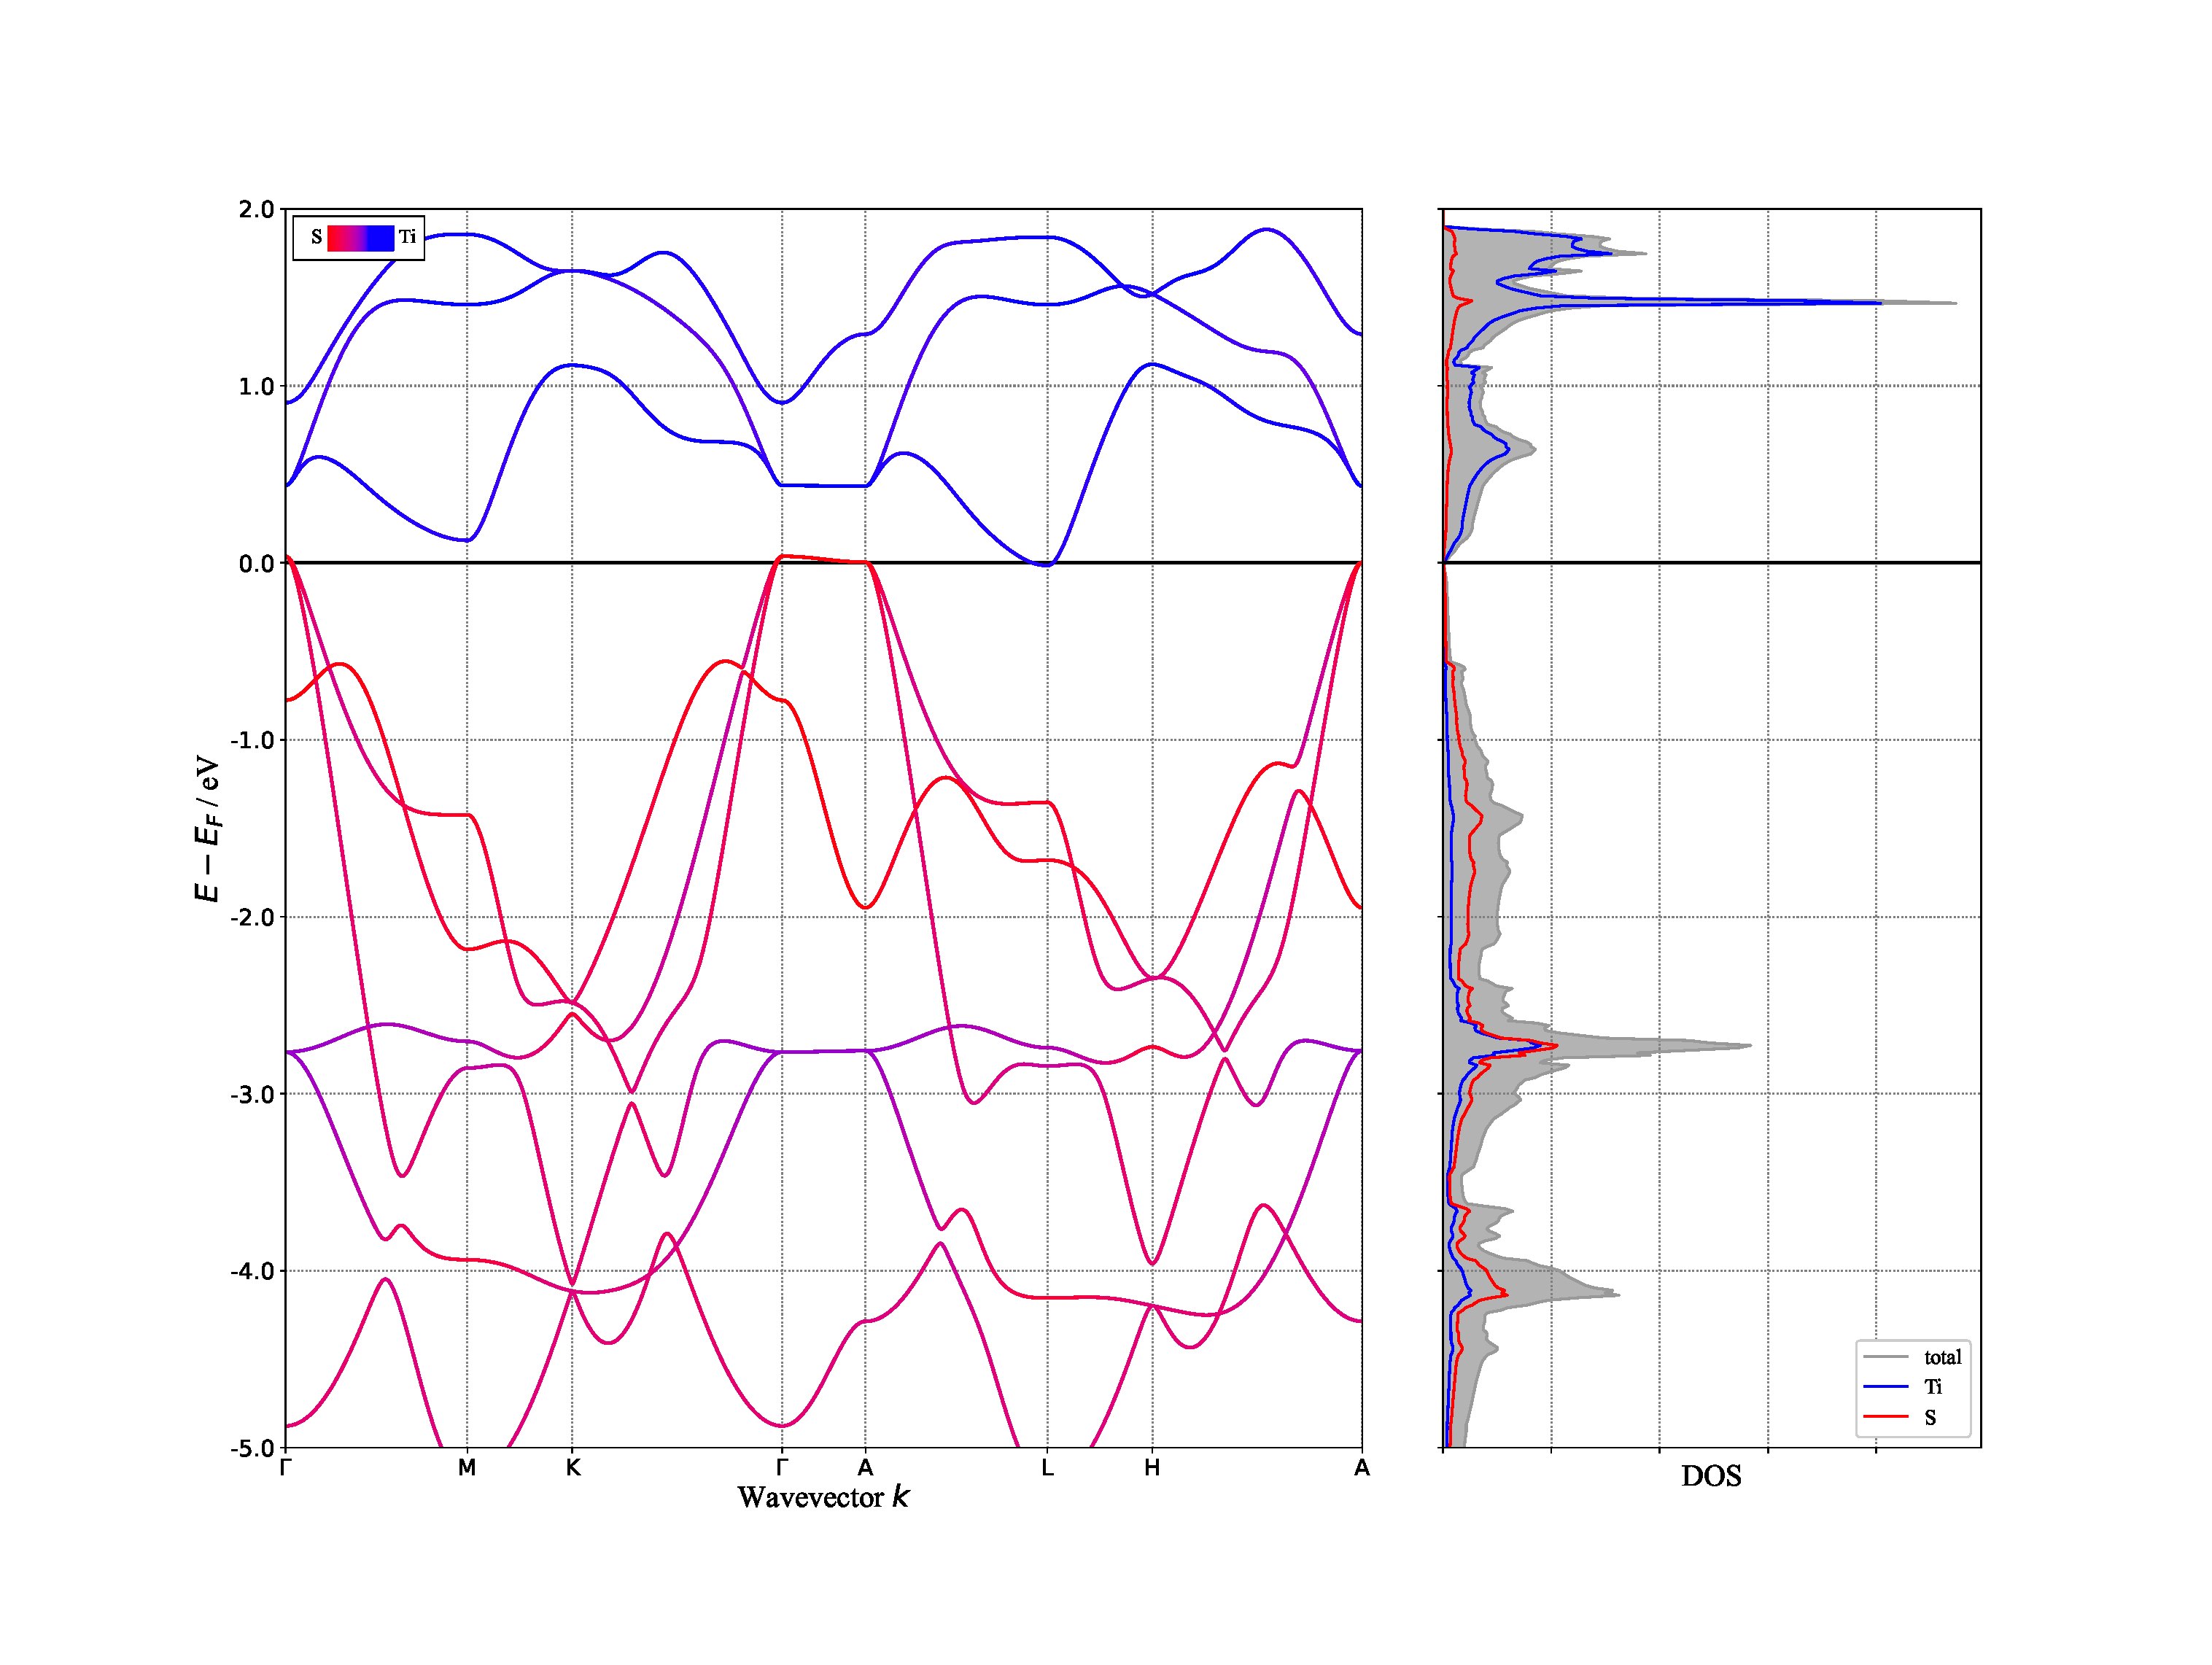
\includegraphics[width=\linewidth]{img/results/TiS2_GGA_relaxed_BAND+DOS.eps}
    	\caption{TiS2}
	\end{subfigure}
	\begin{subfigure}[b]{.4\textwidth}
    	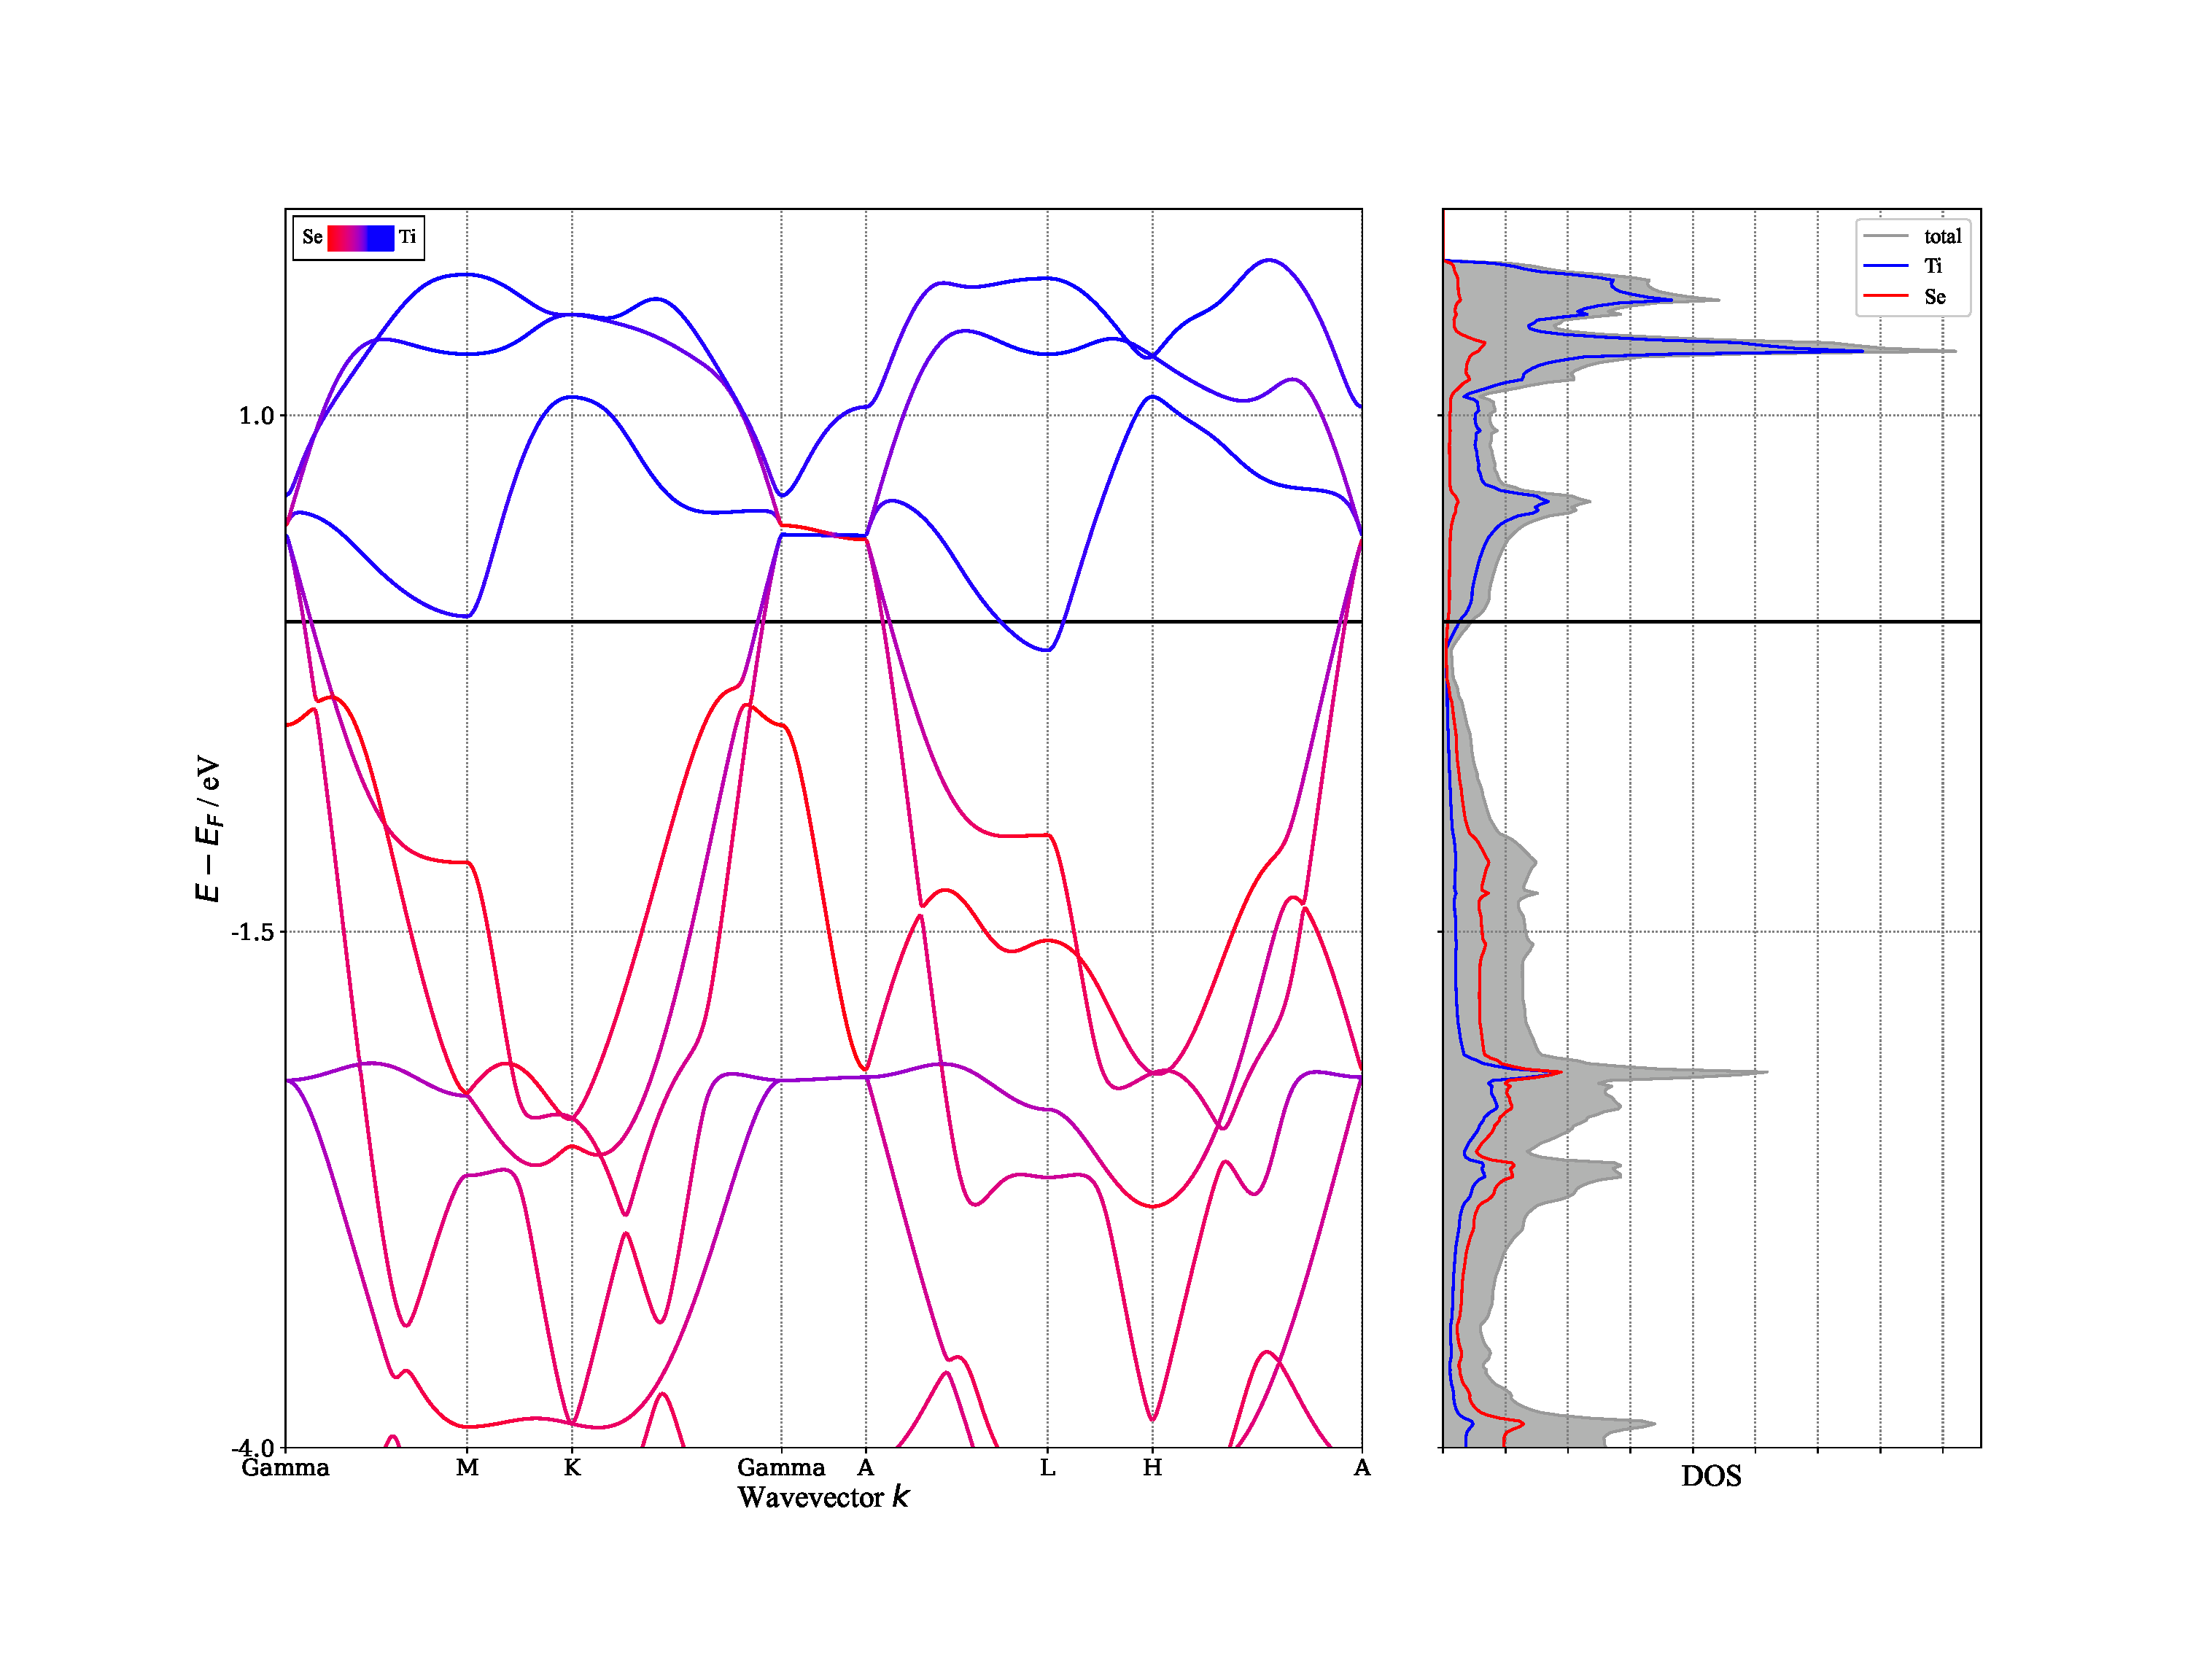
\includegraphics[width=\linewidth]{img/results/TiSe2_GGA_relaxed_BAND+DOS.eps}
    	\caption{
    	TiSe2}
	\end{subfigure}
	\begin{subfigure}[b]{.4\textwidth}
    	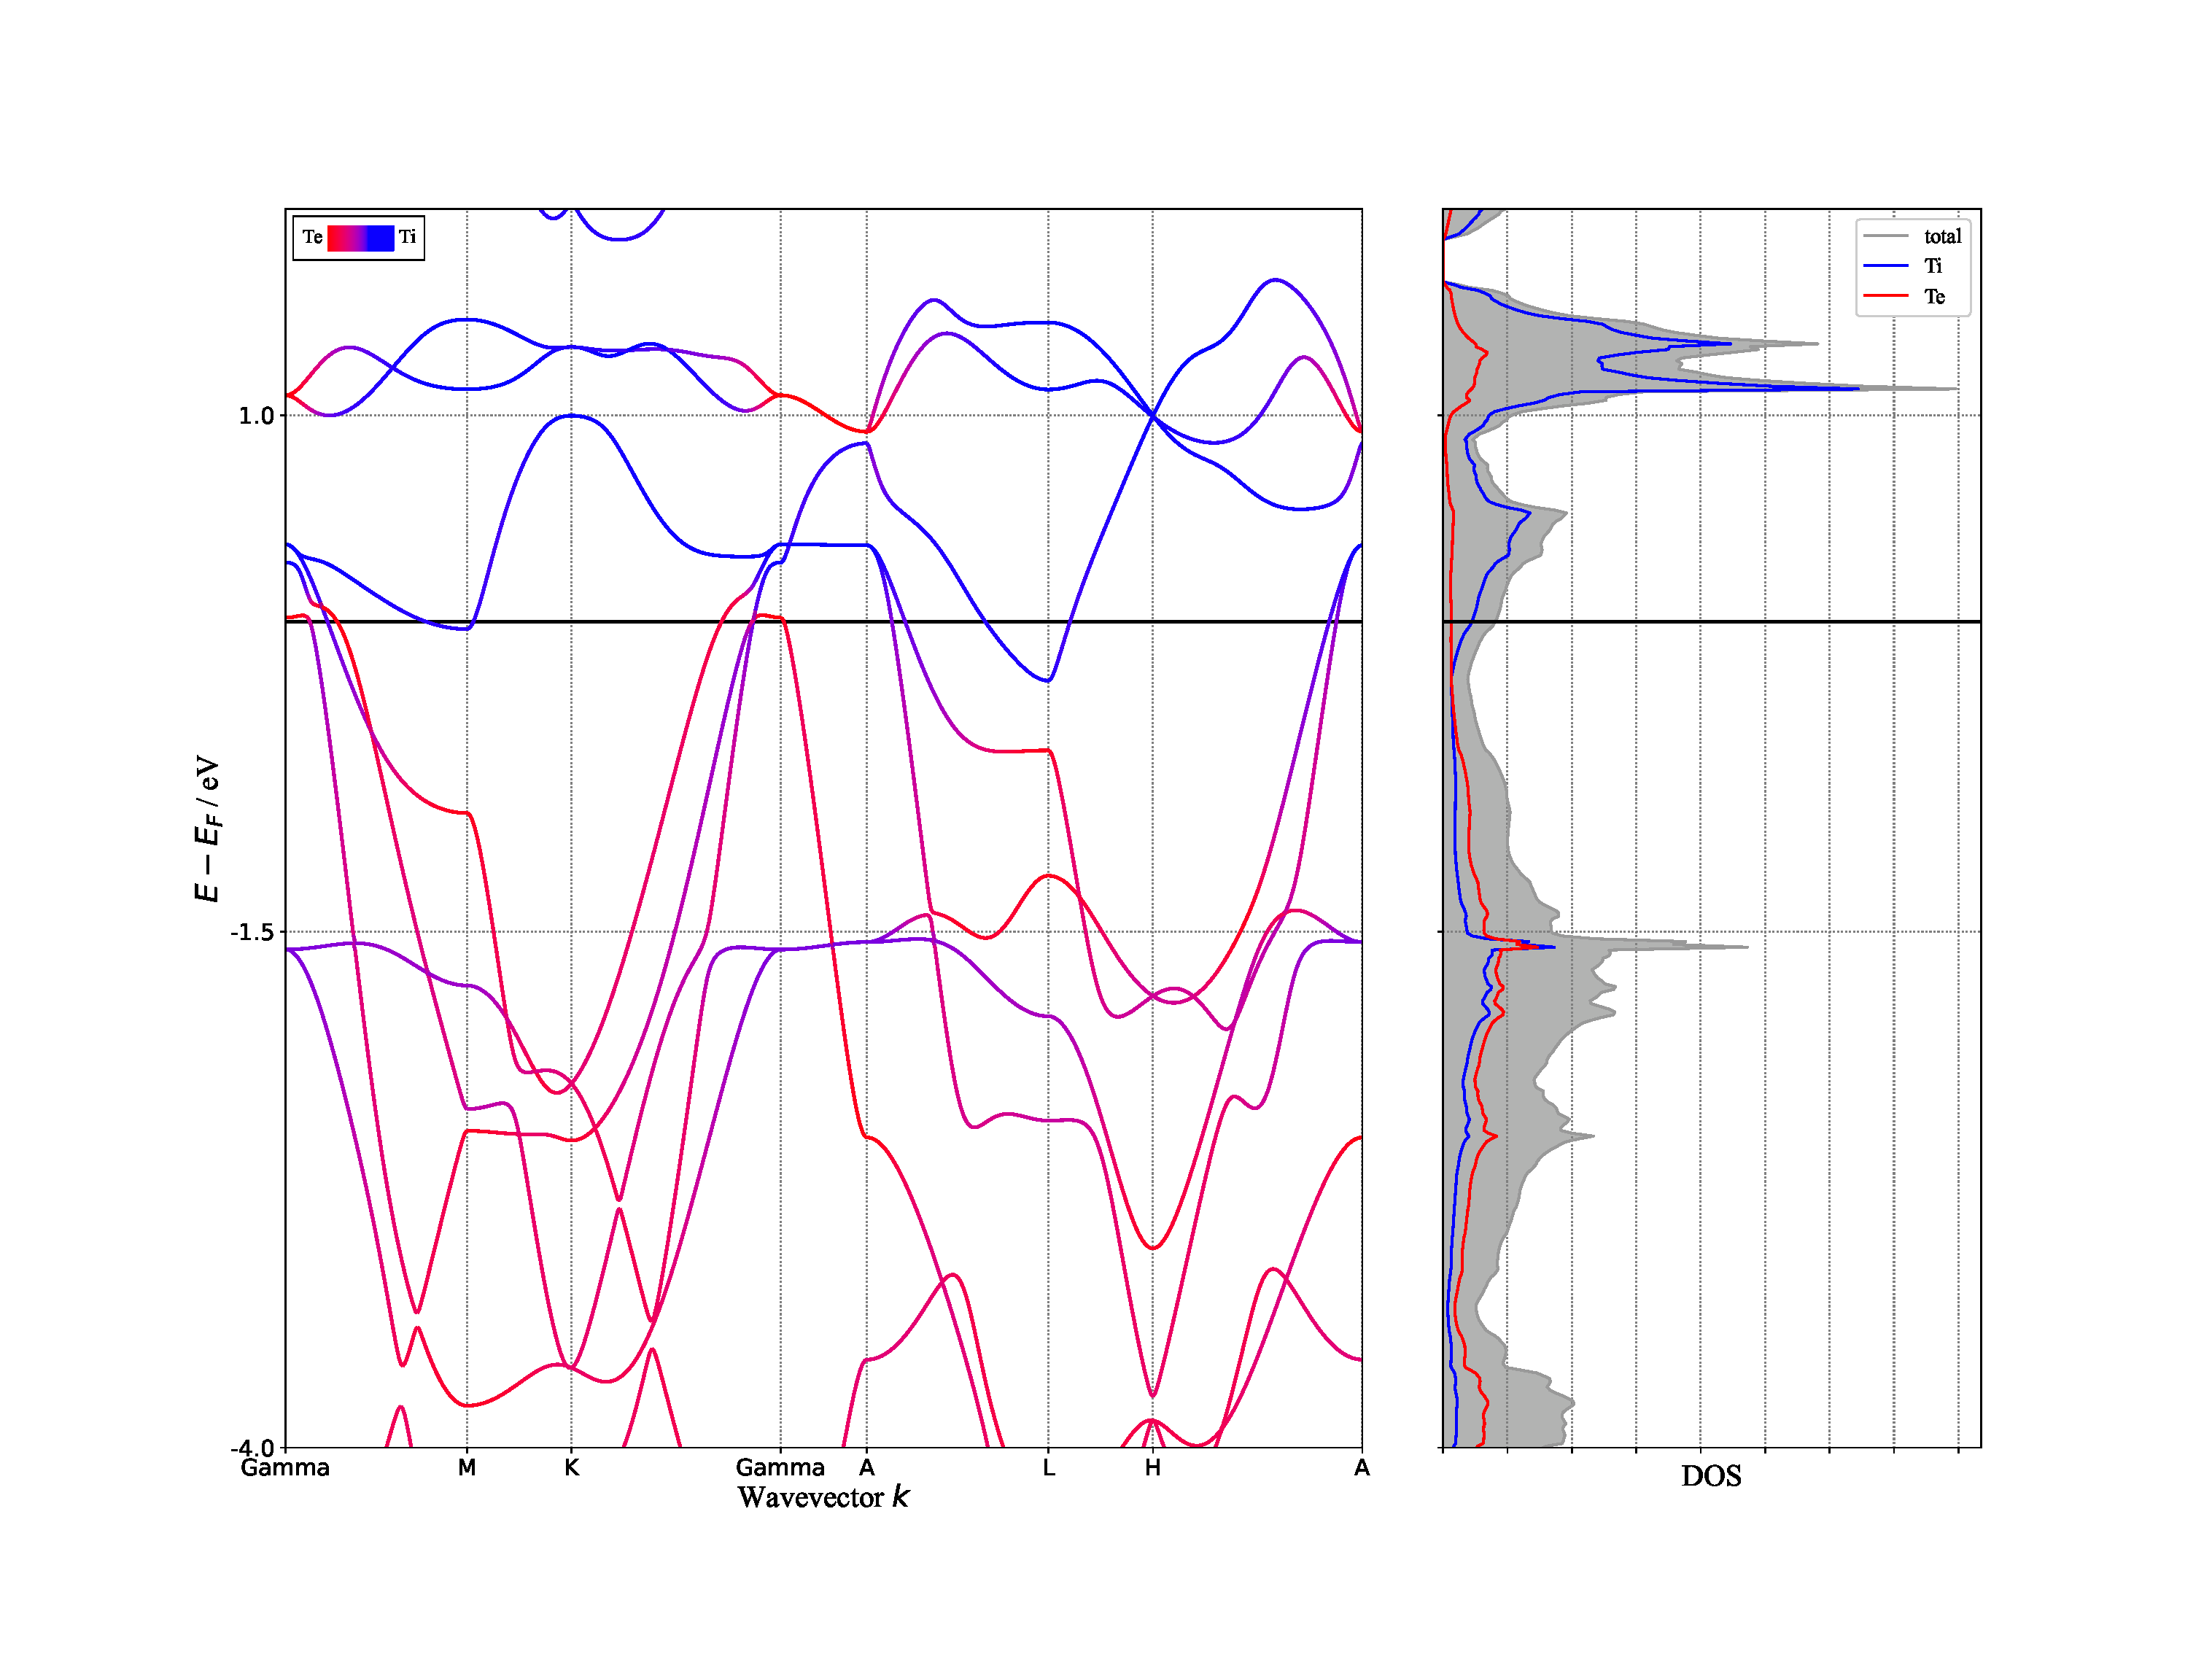
\includegraphics[width=\linewidth]{img/results/TiTe2_GGA_relaxed_BAND+DOS.eps}
    	\caption{
    	TiTe2}
	\end{subfigure}
\caption{Електронна будова TiS$_2$, TiSe$_2$, TiTe$_2$ червоним кольором позначено вклад атомів халькогену (S, Se, Te) синім атомів металу (Ti), розрахована з GGA.}
\label{fig:bandstructireGGA}
\end{figure}

Було визначено що при використані GGA PBE функціоналу, як і очікувалось, відображає зону структуру, що схожа на компенсований метал див. рис. \ref{fig:bandstructireGGA}. На малюнку \ref{fig:fermisurf}, як раз можна побачити, що об'єм електронних карманів приблизно дорівнює об'єму дірок.

\begin{figure}[H]
\centering
	\begin{subfigure}[b]{.4\textwidth}
    	\includegraphics[width=\linewidth]{img/results/fstite2.pdf}
    	\caption{TiTe2}
	\end{subfigure}
	\begin{subfigure}[b]{.4\textwidth}
    	\includegraphics[width=\linewidth]{img/results/fstise2.pdf}
    	\caption{
    	TiSe2}
	\end{subfigure}
	\begin{subfigure}[b]{.9\textwidth}
    	\includegraphics[width=\linewidth]{img/results/fstis2.pdf}
    	\caption{
    	TiS2}
	\end{subfigure}
\caption{Розрахована поверхня фермі TiS$_2$, TiSe$_2$, TiTe$_2$ за допомогою PBE GGA функціоналу}
\label{fig:fermisurf}
\end{figure}

Після цього було задіяно SCAN функціонал та отримано наступні результати див. мал. \ref{fig:bandstructireSCAN}. Зоні спектри дуже схожі які були розраховані у GGA наближені. Але все ж завдяки тому що SCAN більш точно описує електрону будову ван-дер-Ваальсових матеріалів. То все ж таки перекриття у точці $L$ значно зменшується та становить вже -0.0286 eV. -- в $\approx$ 2 менше в порівняні з -0.0633 eV. у GGA. 

\begin{figure}[H]
\centering
	\begin{subfigure}[b]{.9\textwidth}
    	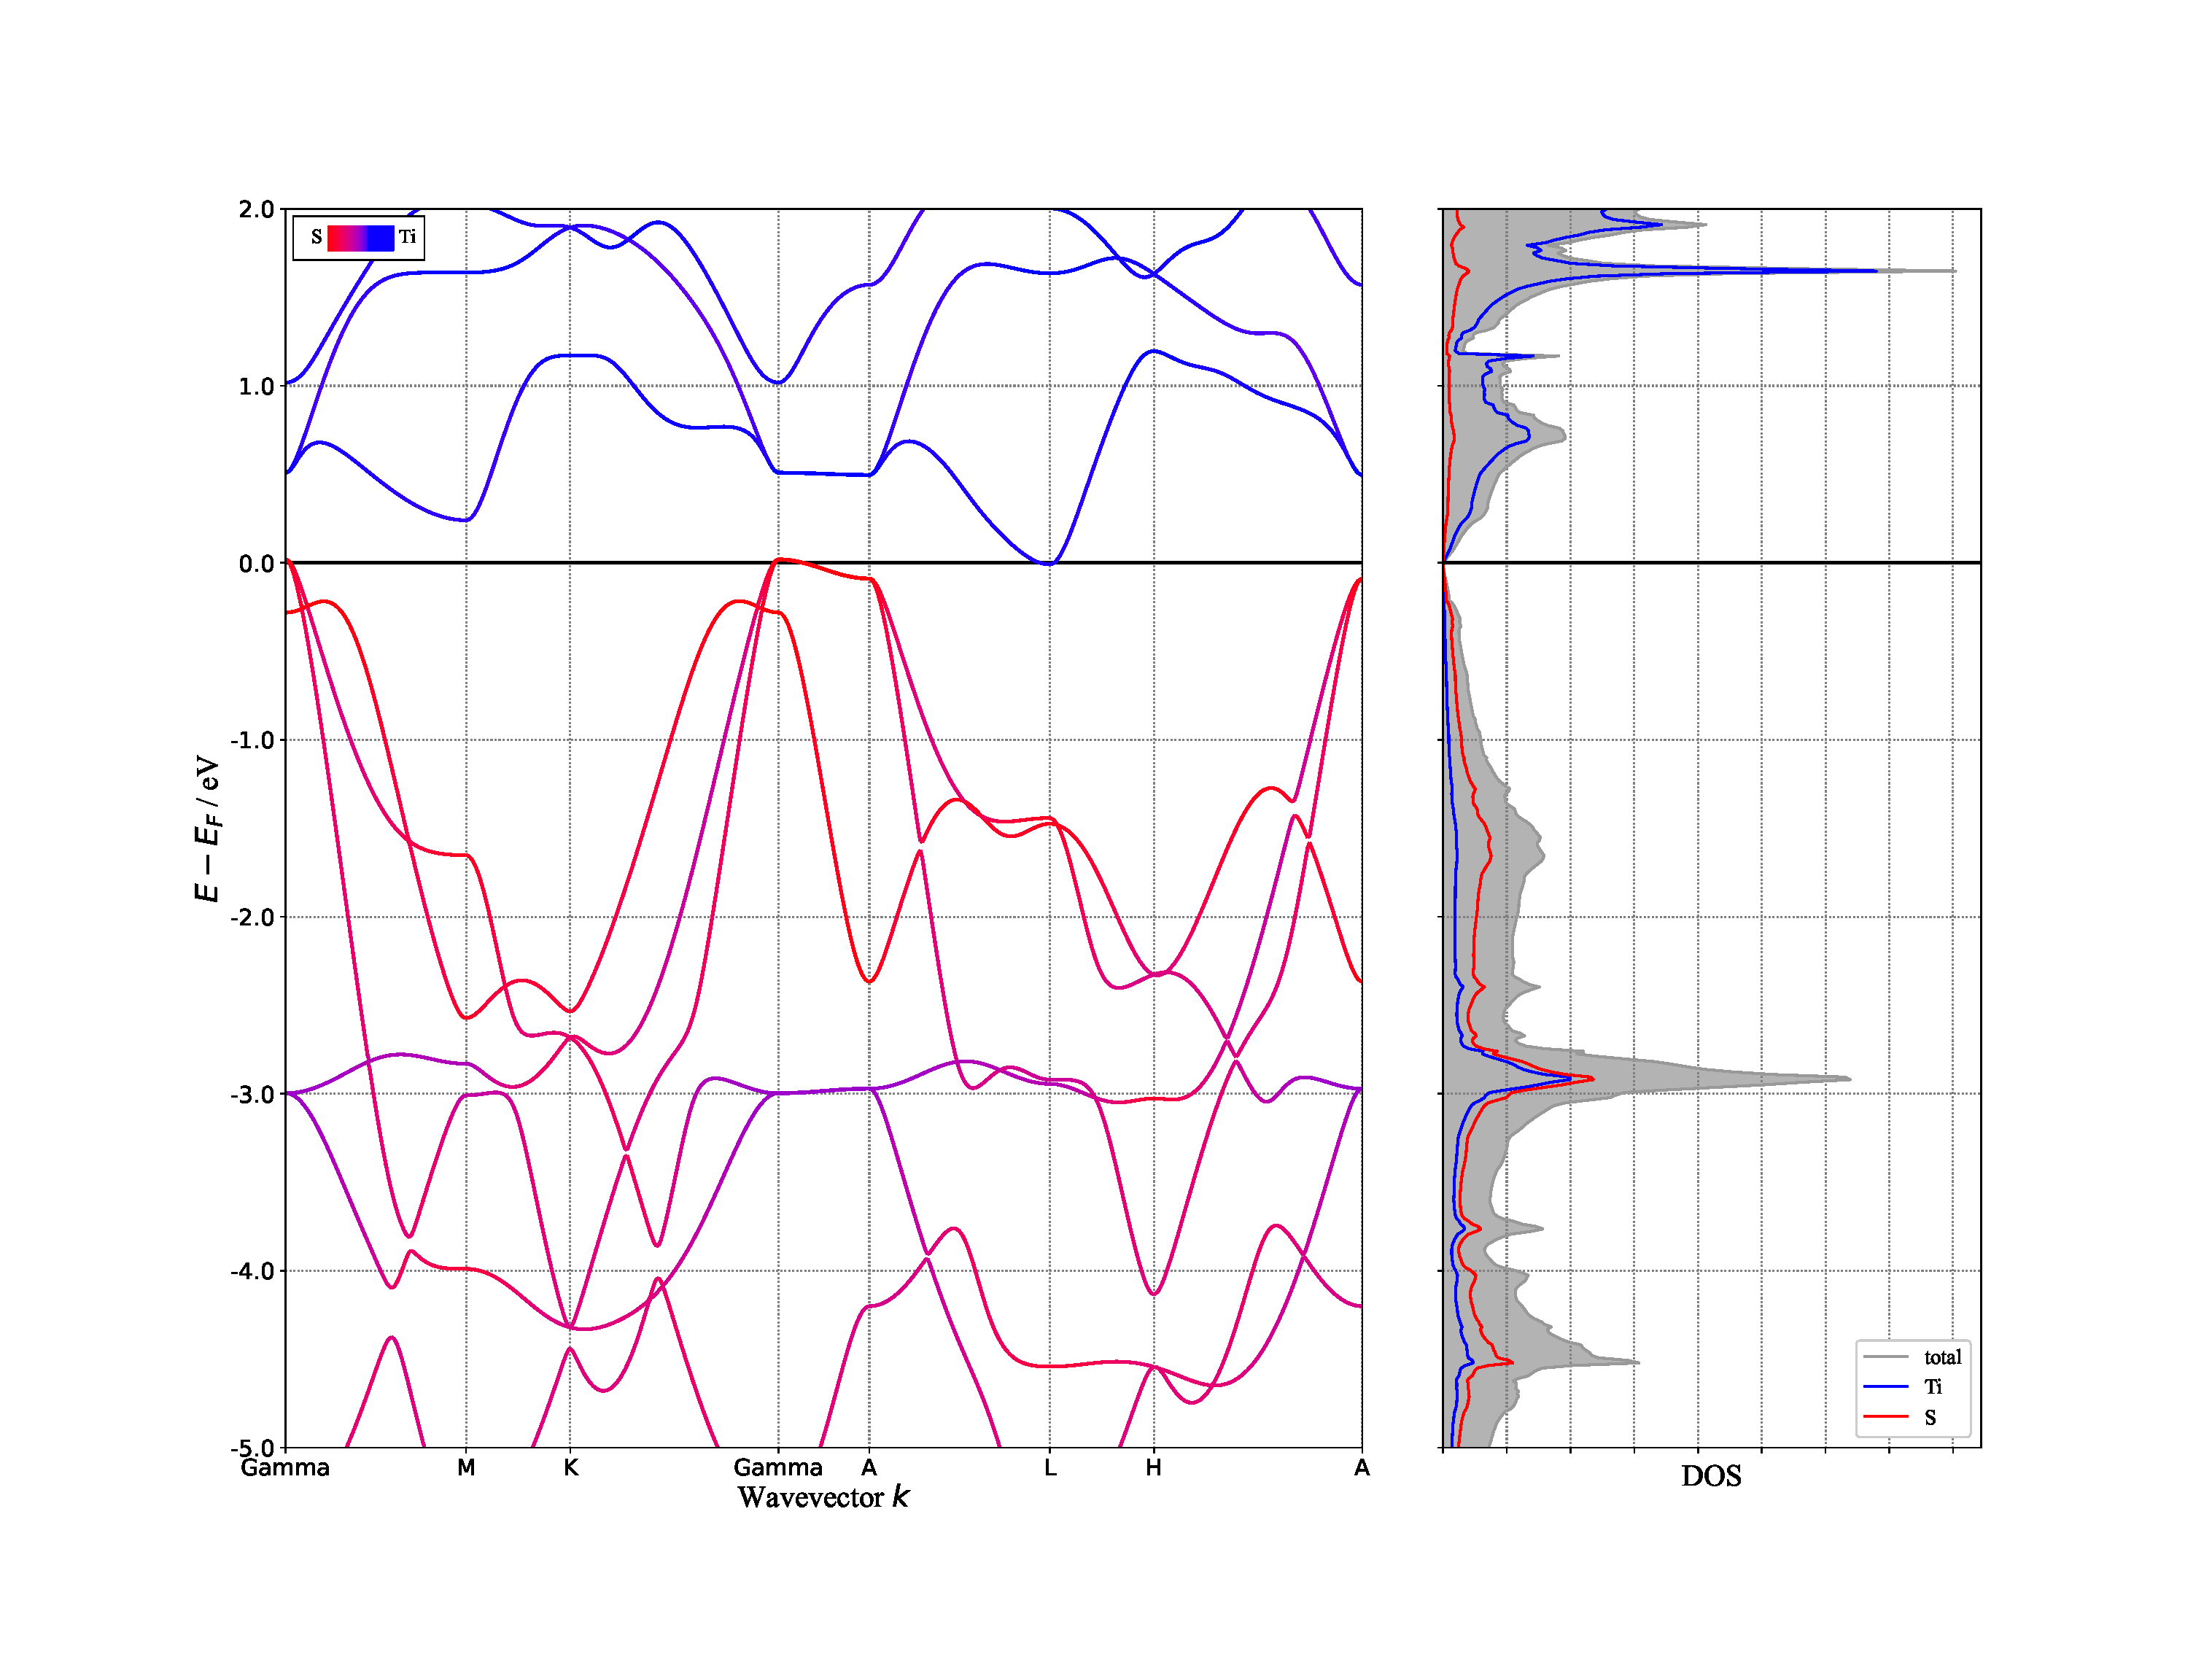
\includegraphics[width=\linewidth]{img/results/TiS2_SCAN_relaxed_BAND+DOS.eps}
    	\caption{TiS2}
	\end{subfigure}
	\begin{subfigure}[b]{.4\textwidth}
    	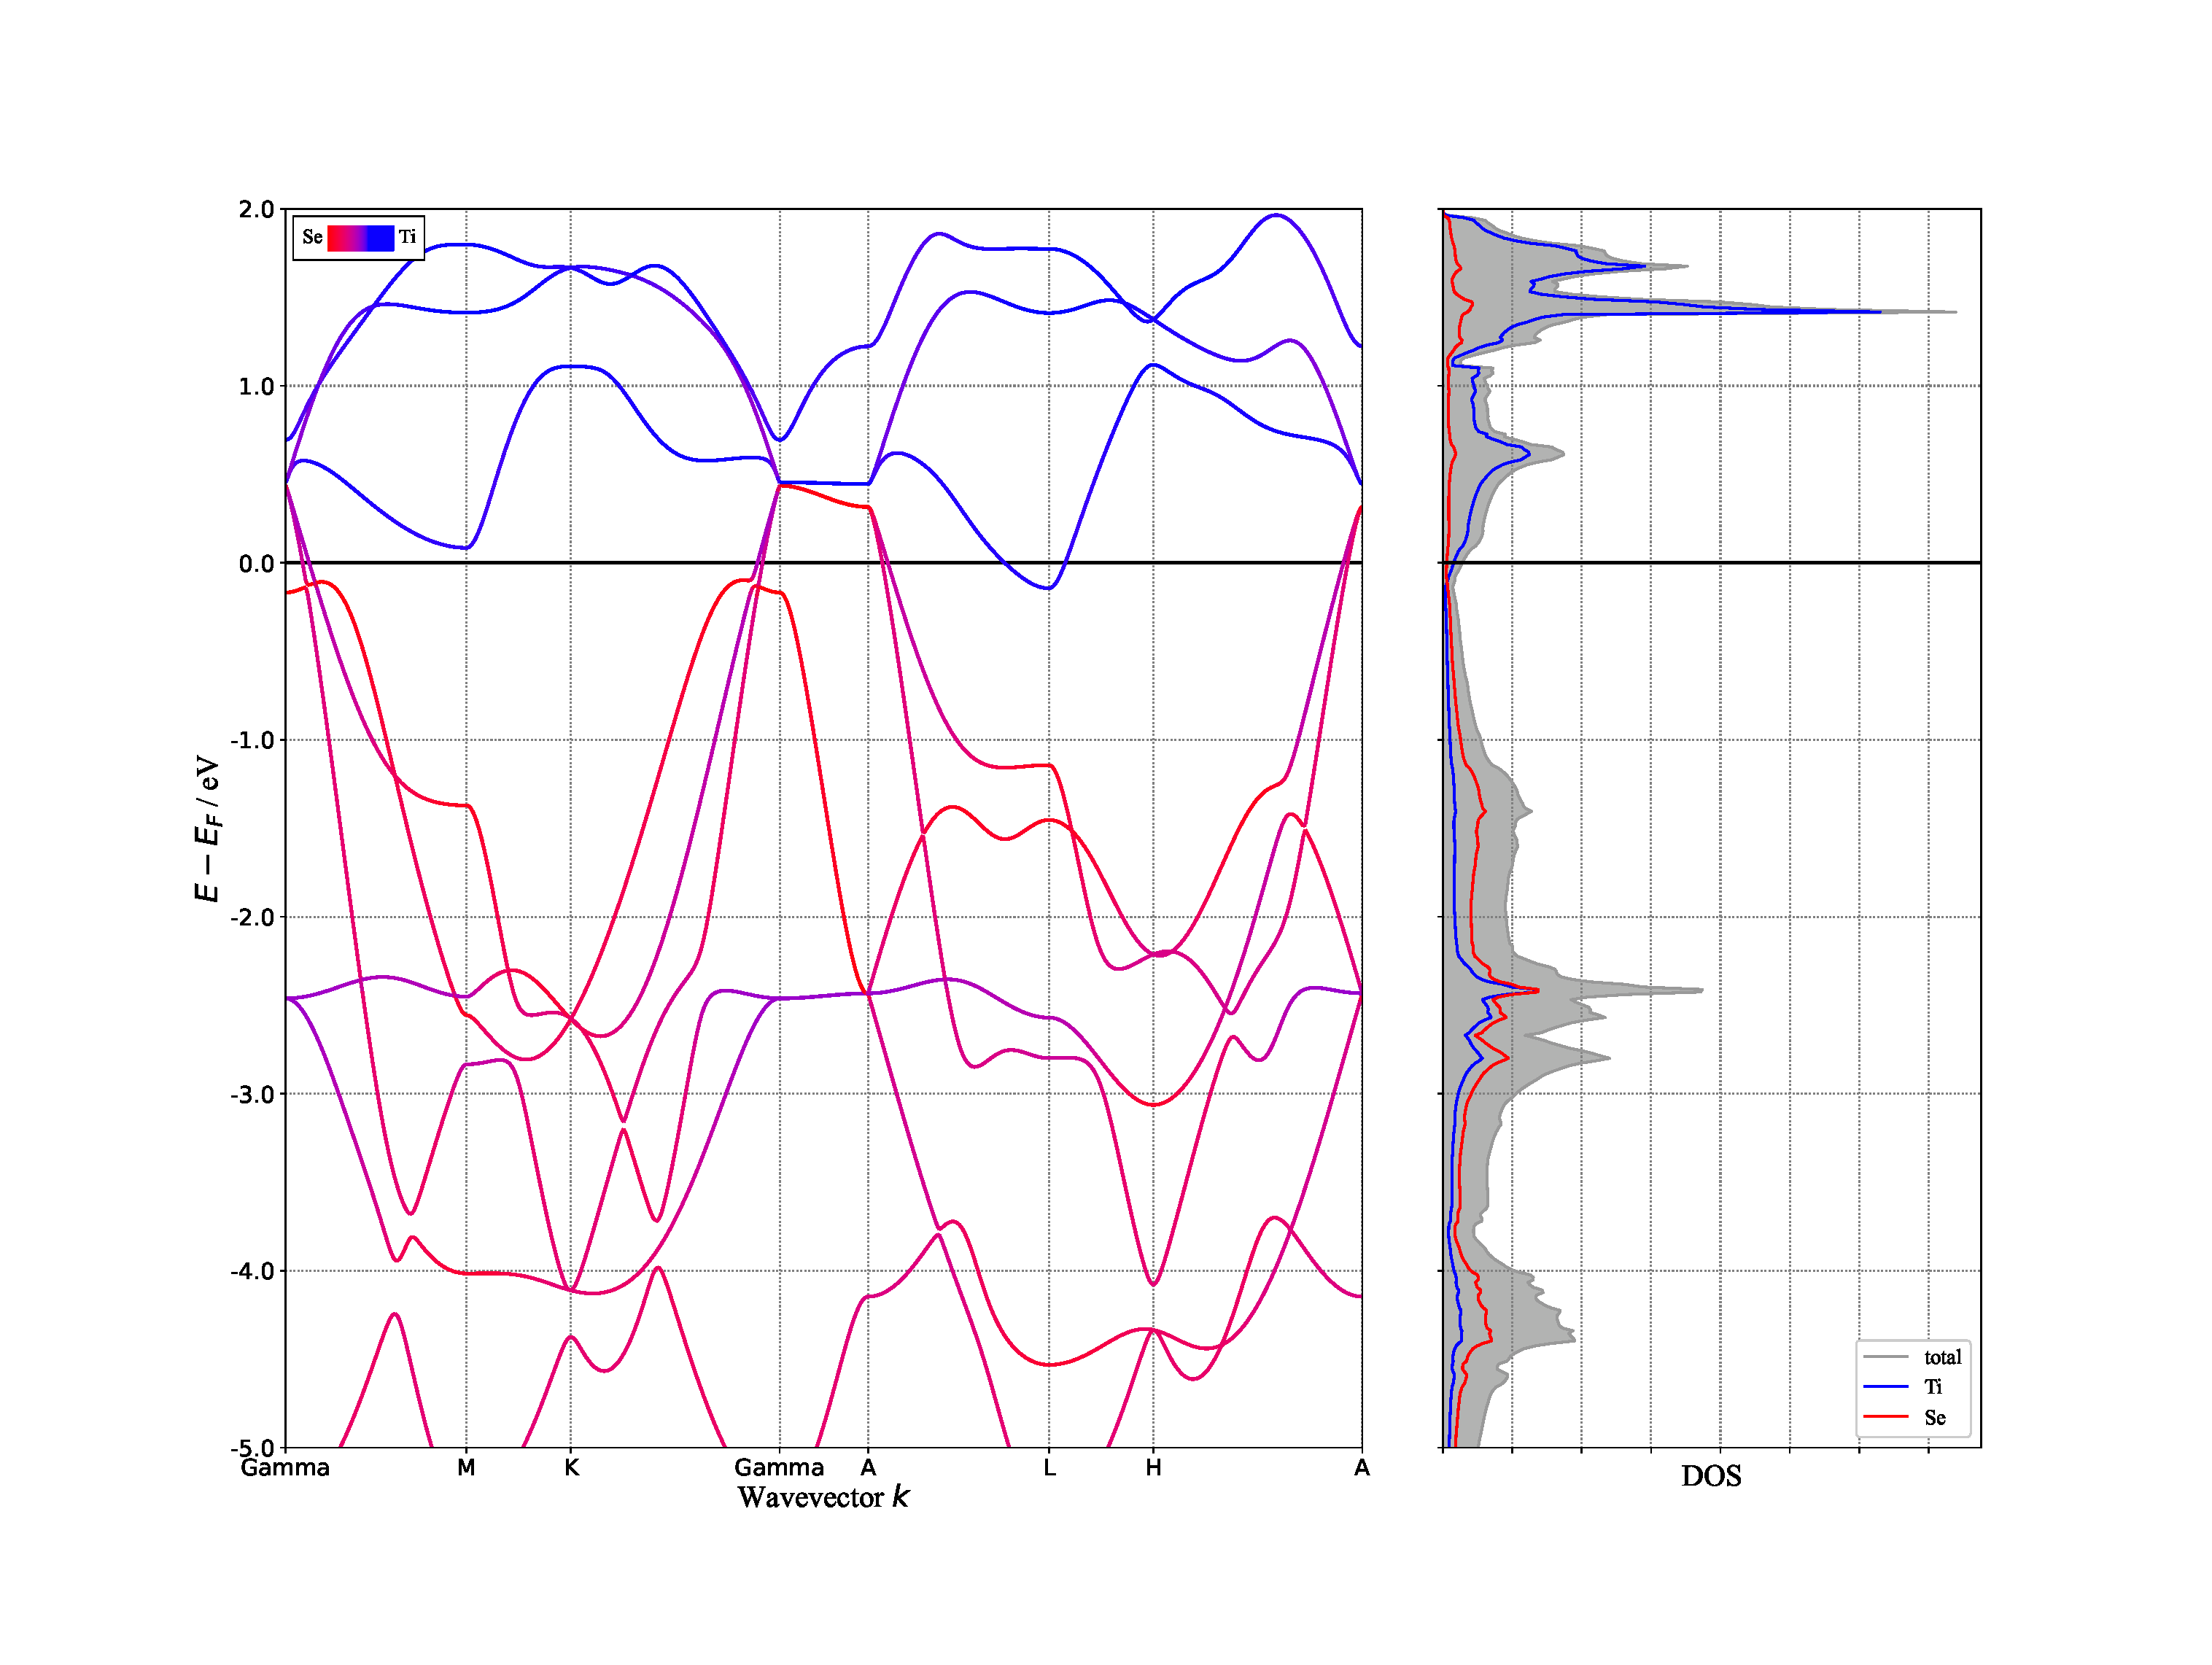
\includegraphics[width=\linewidth]{img/results/TiSe2_SCAN_relaxed_BAND+DOS}
    	\caption{
    	TiSe2}
	\end{subfigure}
	\begin{subfigure}[b]{.4\textwidth}
    	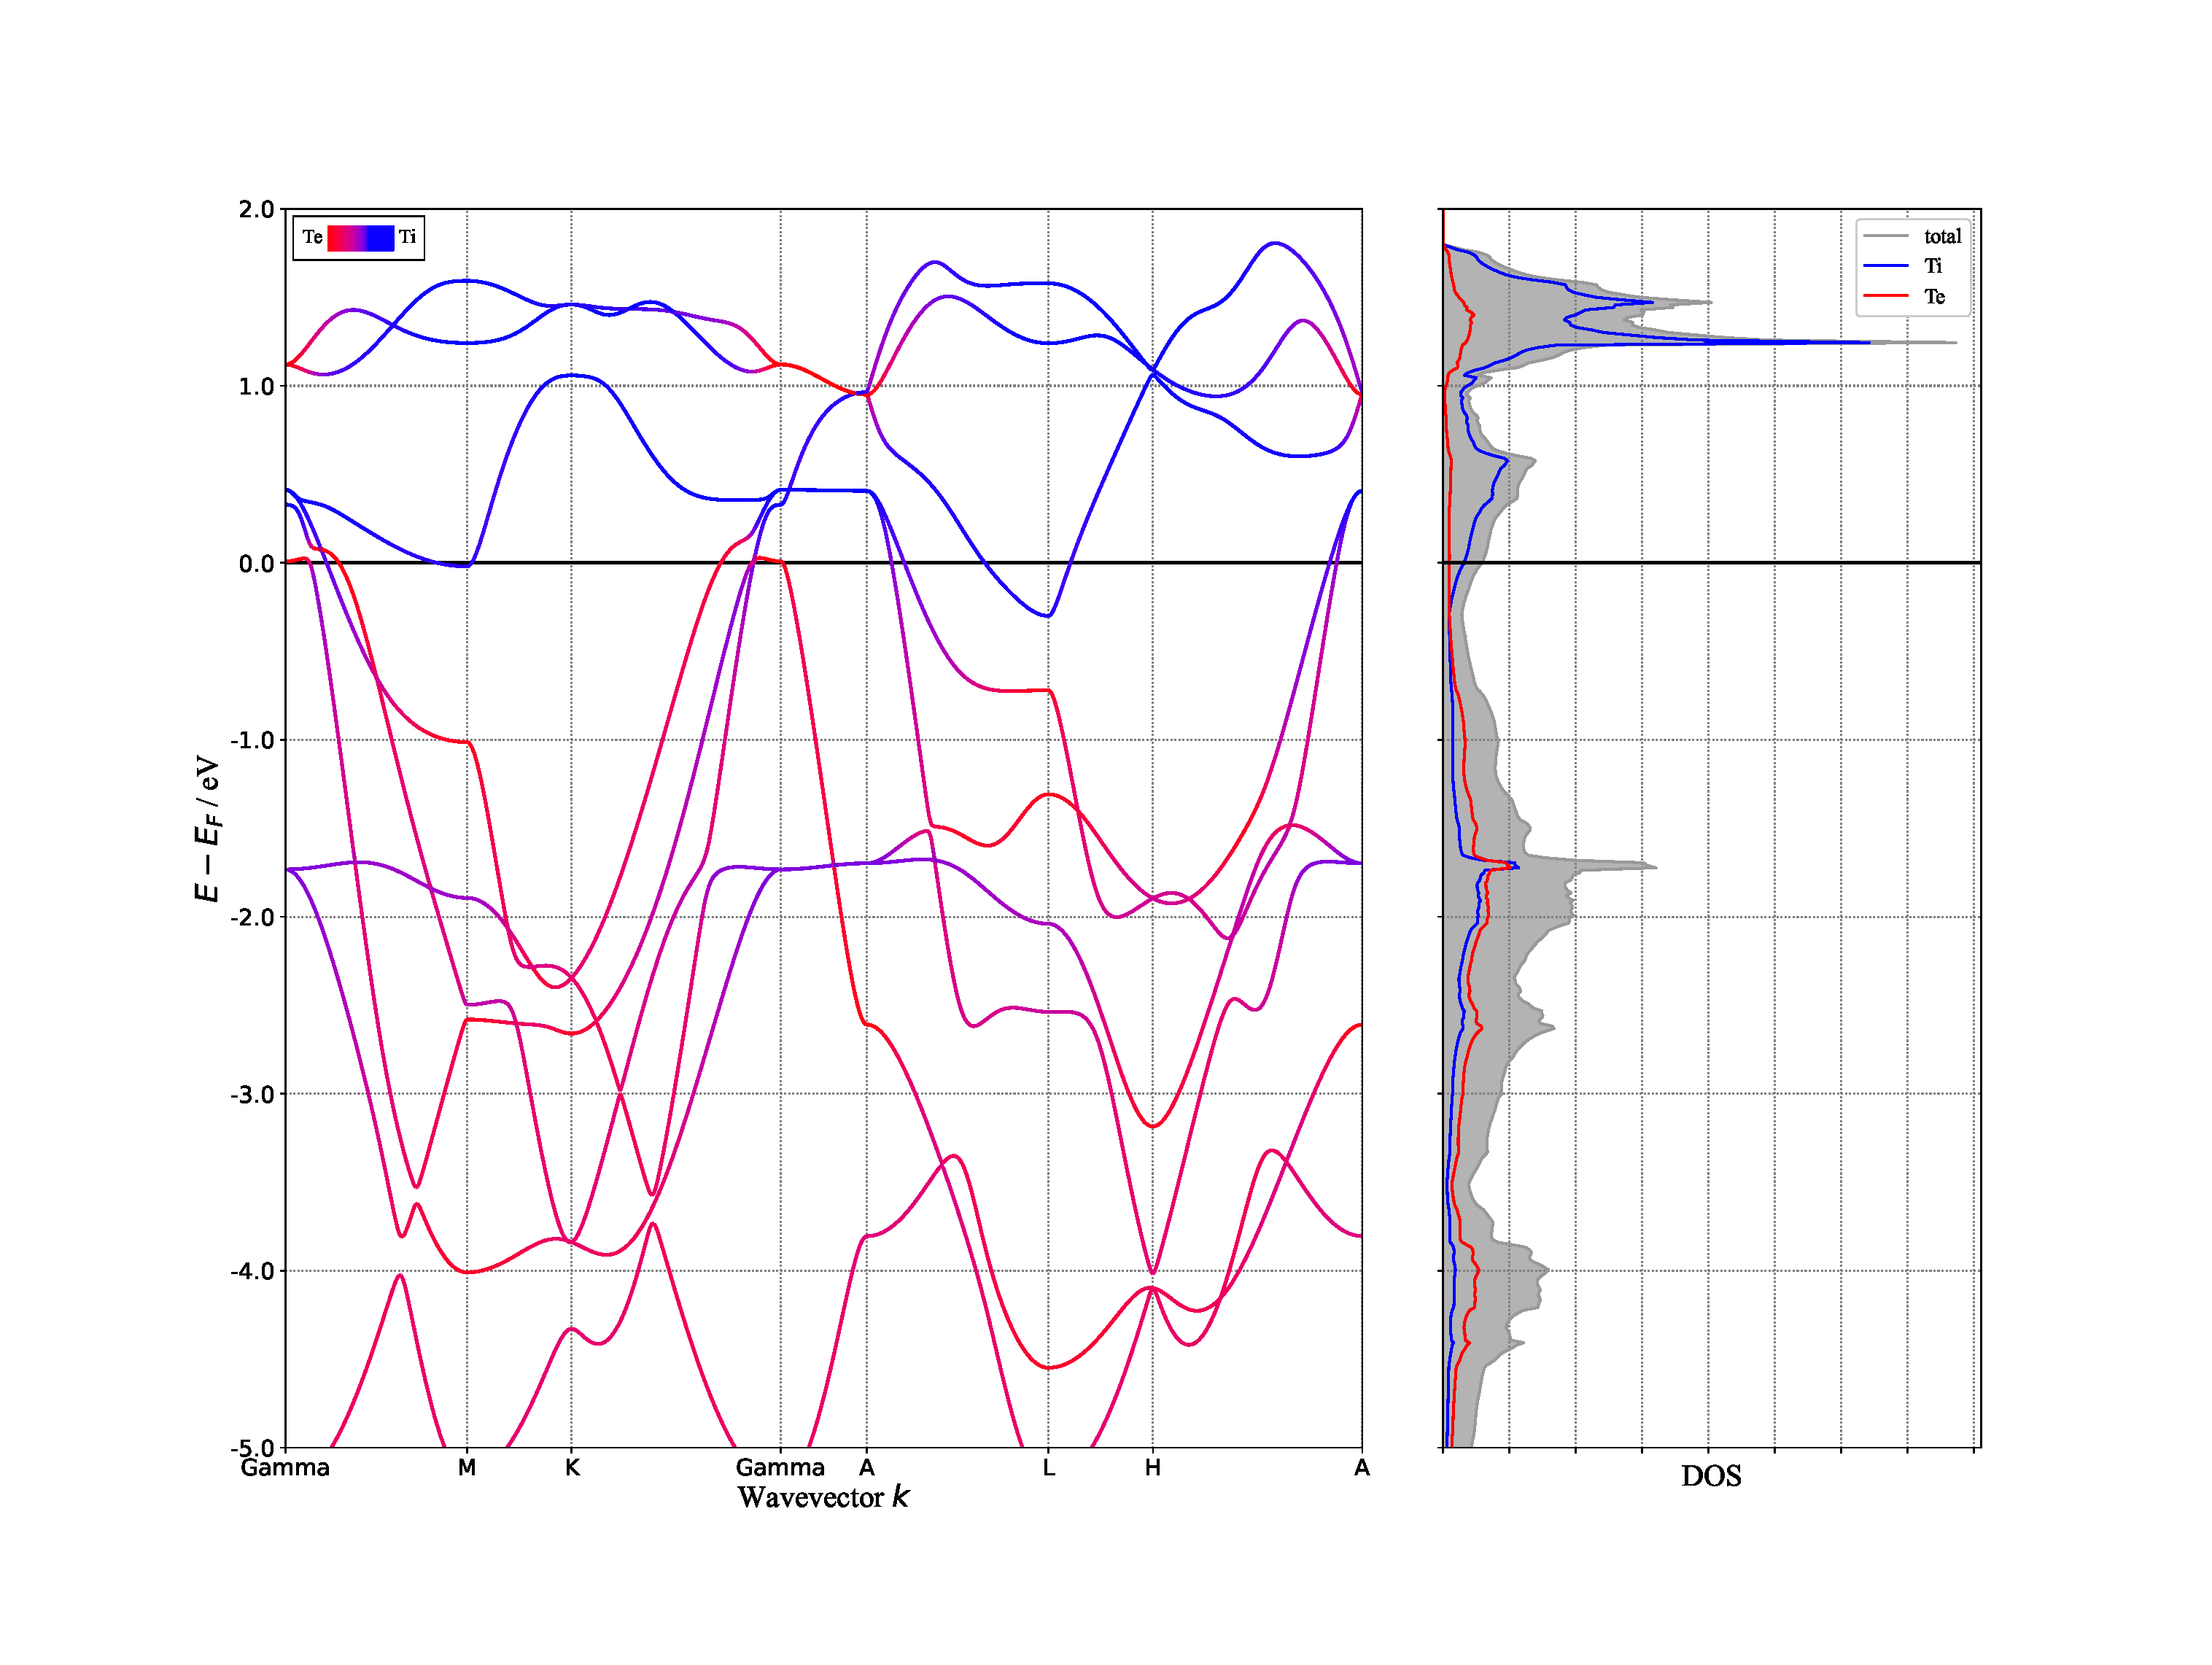
\includegraphics[width=\linewidth]{img/results/TiTe2_SCAN_relaxed_BAND+DOS}
    	\caption{
    	TiTe2}
	\end{subfigure}
\caption{Електронна будова TiS$_2$, TiSe$_2$, TiTe$_2$ червоним кольором позначено вклад атомів халькогену (S, Se, Te) синім атомів металу (Ti), розрахована з SCAN.}
\label{fig:bandstructireSCAN}
\end{figure}

Для того щоб показати наскільки матеріал сильно корельований ми за референс брали саме TiS$_2$ сполуку, закріпляли координати атомів елементарної комірки та варіювали U до 3.0 eV \ref{fig:variationU_GGA}. 

\begin{figure}
	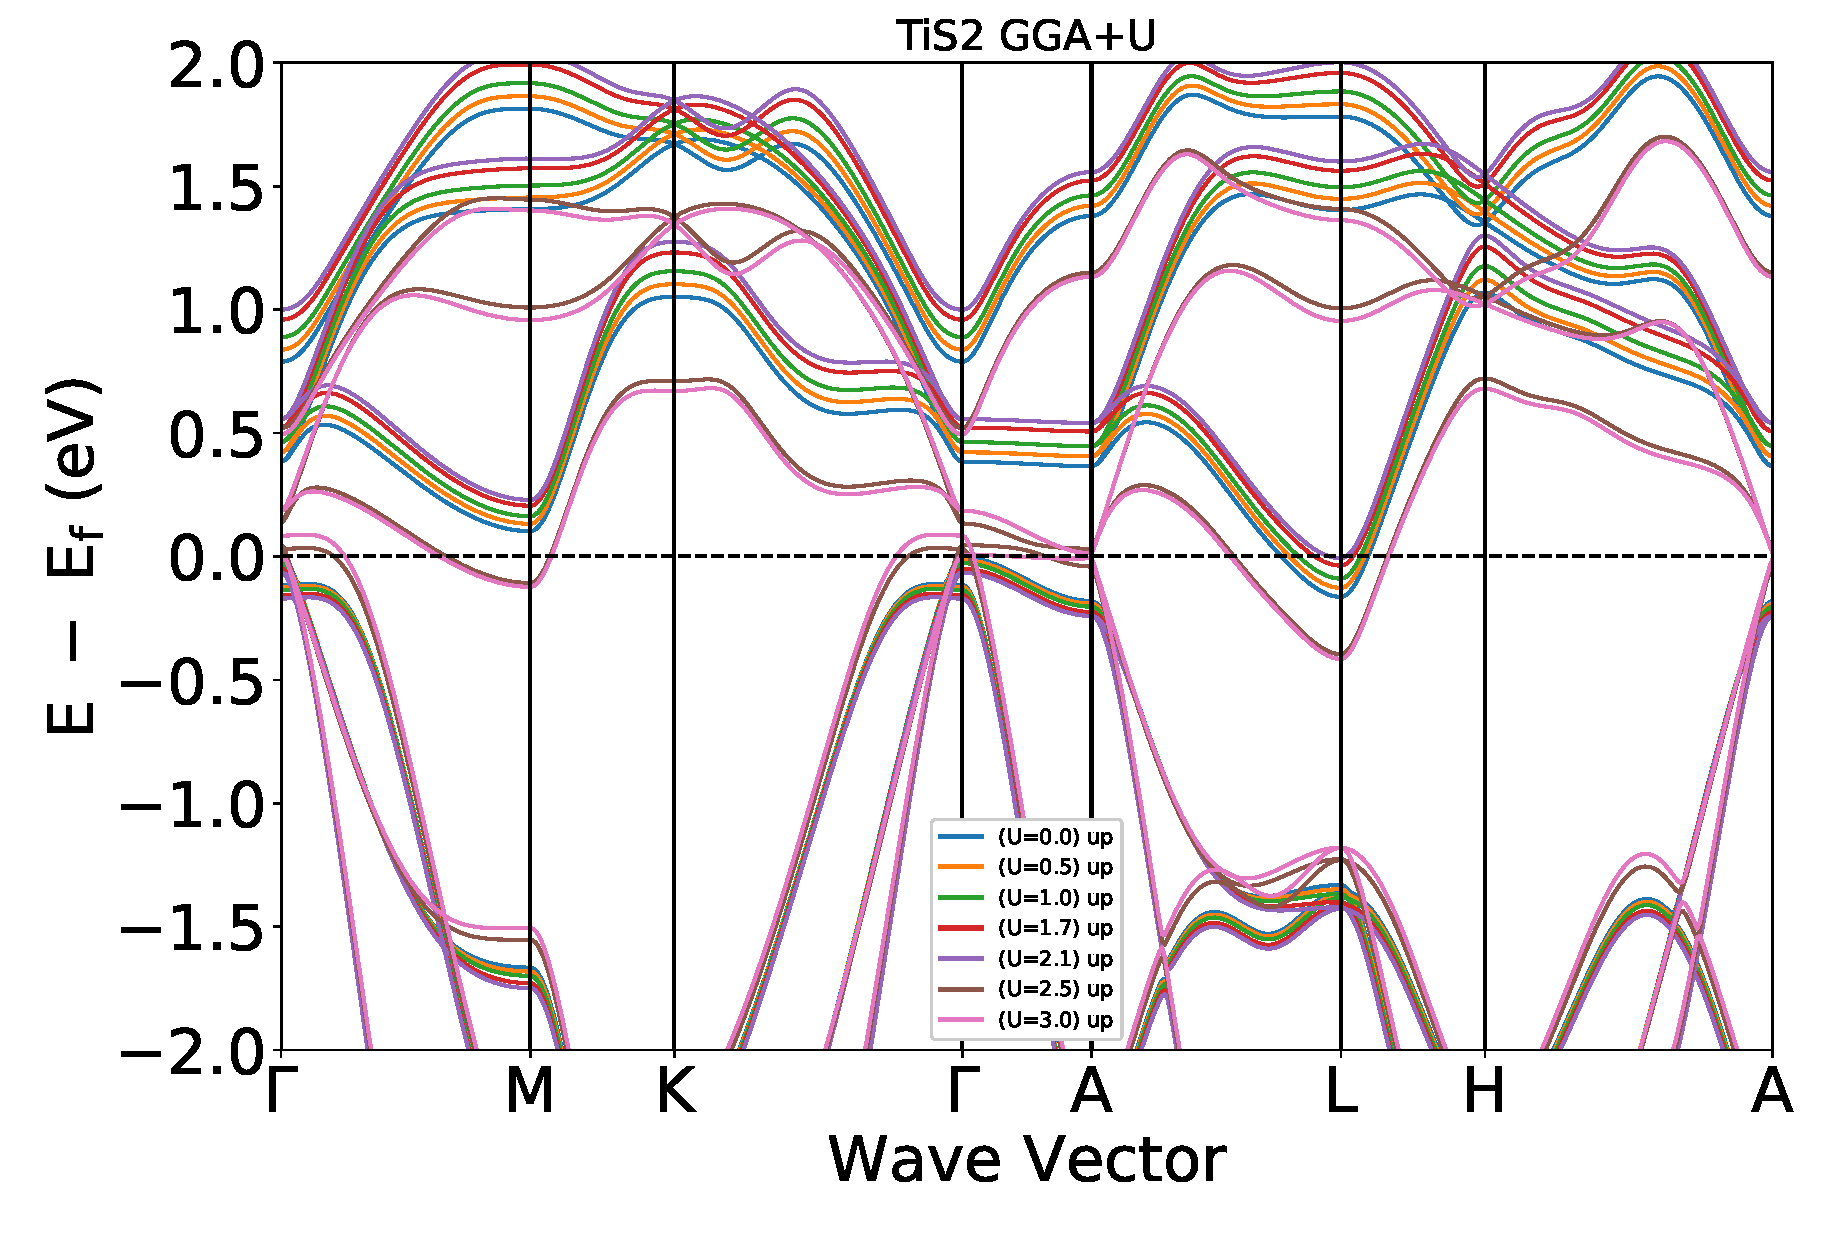
\includegraphics[scale=0.6]{results/TiS2_GGA+U--variation.eps}
	\caption{Зона структура при варіації U від 0 до 3.0 eV, для TiS$_2$}
	\label{fig:variationU_GGA}
\end{figure}

Як зазначалось у попередніх розділах, для опису сильнокорельованих систем ми маємо використовувати DFT+U. При прикладених U зонна щілина відкривається таб. \ref{tab:VariationU} на 0.0129 eV. при $U=1.7$ та 0.0587 eV. при $U=2.1$, але цього не достатньо, щоб чітко стверджувати, ща ми маємо напівпровідникову поведінку матеріалу. 

\begin{table}[H]\centering
\scriptsize
\begin{tabular}{lrr}\toprule
\multicolumn{2}{c}{\textbf{Варіація U }} \\\midrule
\multirow{2}{*}{\textbf{U}} &\multirow{2}{*}{\textbf{Band Gap}} \\
& \\
0.0 & -0.1609 \\
0.5 &-0.1134 \\
1.0 &-0.0631 \\
1.7 &0.0129 \\
2.1 &0.0587 \\
2.5 &-0.4422 \\
3.0 &-0.5039 \\
\bottomrule
\end{tabular}
\caption{Перетин $p$ орбіталей у точці $L$ з варіацією U для TiS$_2$}\label{tab:VariationU}
\end{table}

Також з даного малюнку, можна побачити, що сама поправка U має немонотонний характер впливу на зону структуру, тобто при деяких значеннях, а саме від $U=2.5$ та $U=3.0$ в нас знову з'являється металевий характер поведінки електронної будови, і що б найбільш дивно -- з'являється перетин між точками $\Gamma-M$, які спостерігаються тільки у сполуках TiSe$_2$ та TiTe$_2$. Це може свідчити про не фізичність використання дуже великих U.

\begin{figure}[H]
	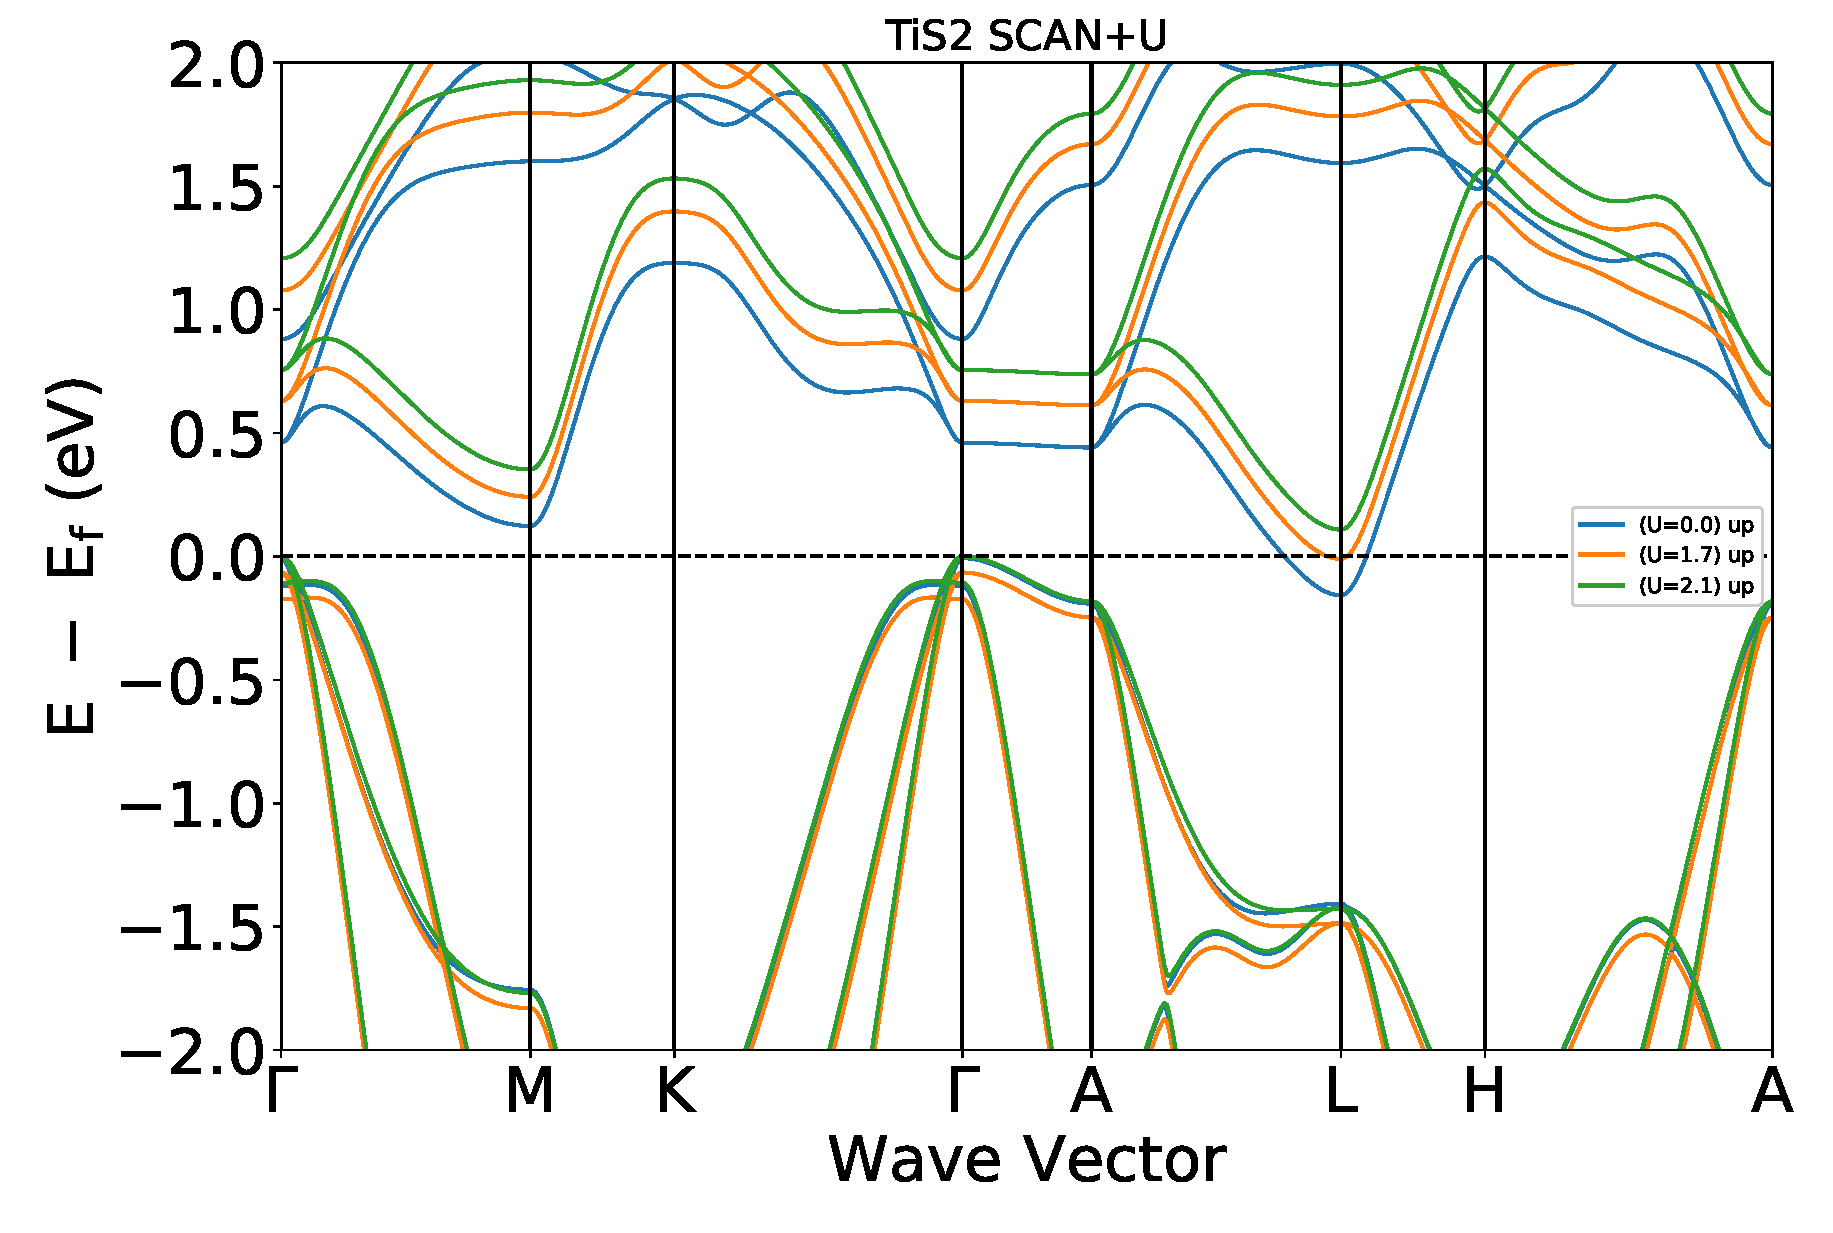
\includegraphics[scale=0.6]{results/TiS2_SCAN+U-variation.eps}
	\caption{Електрона будова TiS$_2$ SCAN + U (U = 0, 1.7, 2.1)}\label{fig:SCAN+U_1.7_2.1}
\end{figure}

Варіюючи U зі значеннями 1.7 eV, 2.1 eV рис. \ref{fig:SCAN+U_1.7_2.1} ми отримуємо щілину при таких самих значеннях, що і при GGA+U, але розмір цієї щілини на відміно від GGA, вже узгоджується з розрахунками іншими методами та експериментами. При використанні функціоналу SCAN+U (U = 2.1 eV) ми бачимо, як відкривається зонна щілина порядку $\approx$ 0.1 eV у сполуці TiS$_2$ див. рис. \ref{fig:SCAN+U_tis2}, але цього не відбувається у TiSe$_2$, TiTe$_2$ див. рис. \ref{fig:SCAN+U_tise2}, \ref{fig:SCAN+U_tite2} і це узгоджується з експериментальними даними.

\begin{figure}[H]
	\includegraphics[scale=0.6]{results/SCAN-rVV10+U}
	\caption{Електронна будова TiS$_2$ з використанням поправок rVV10}\label{fig:rVV10+U}
\end{figure}

Після цього було використано для структурної релаксації ван-дер-Ваальсові поправки \cite{Peng_2016}, які більш краще описують геометрію решітки та отримати вже наближене до експериментального значення щілини $\approx$ 0.22 eV. див. рис. \ref{fig:rVV10+U}

\begin{figure}
	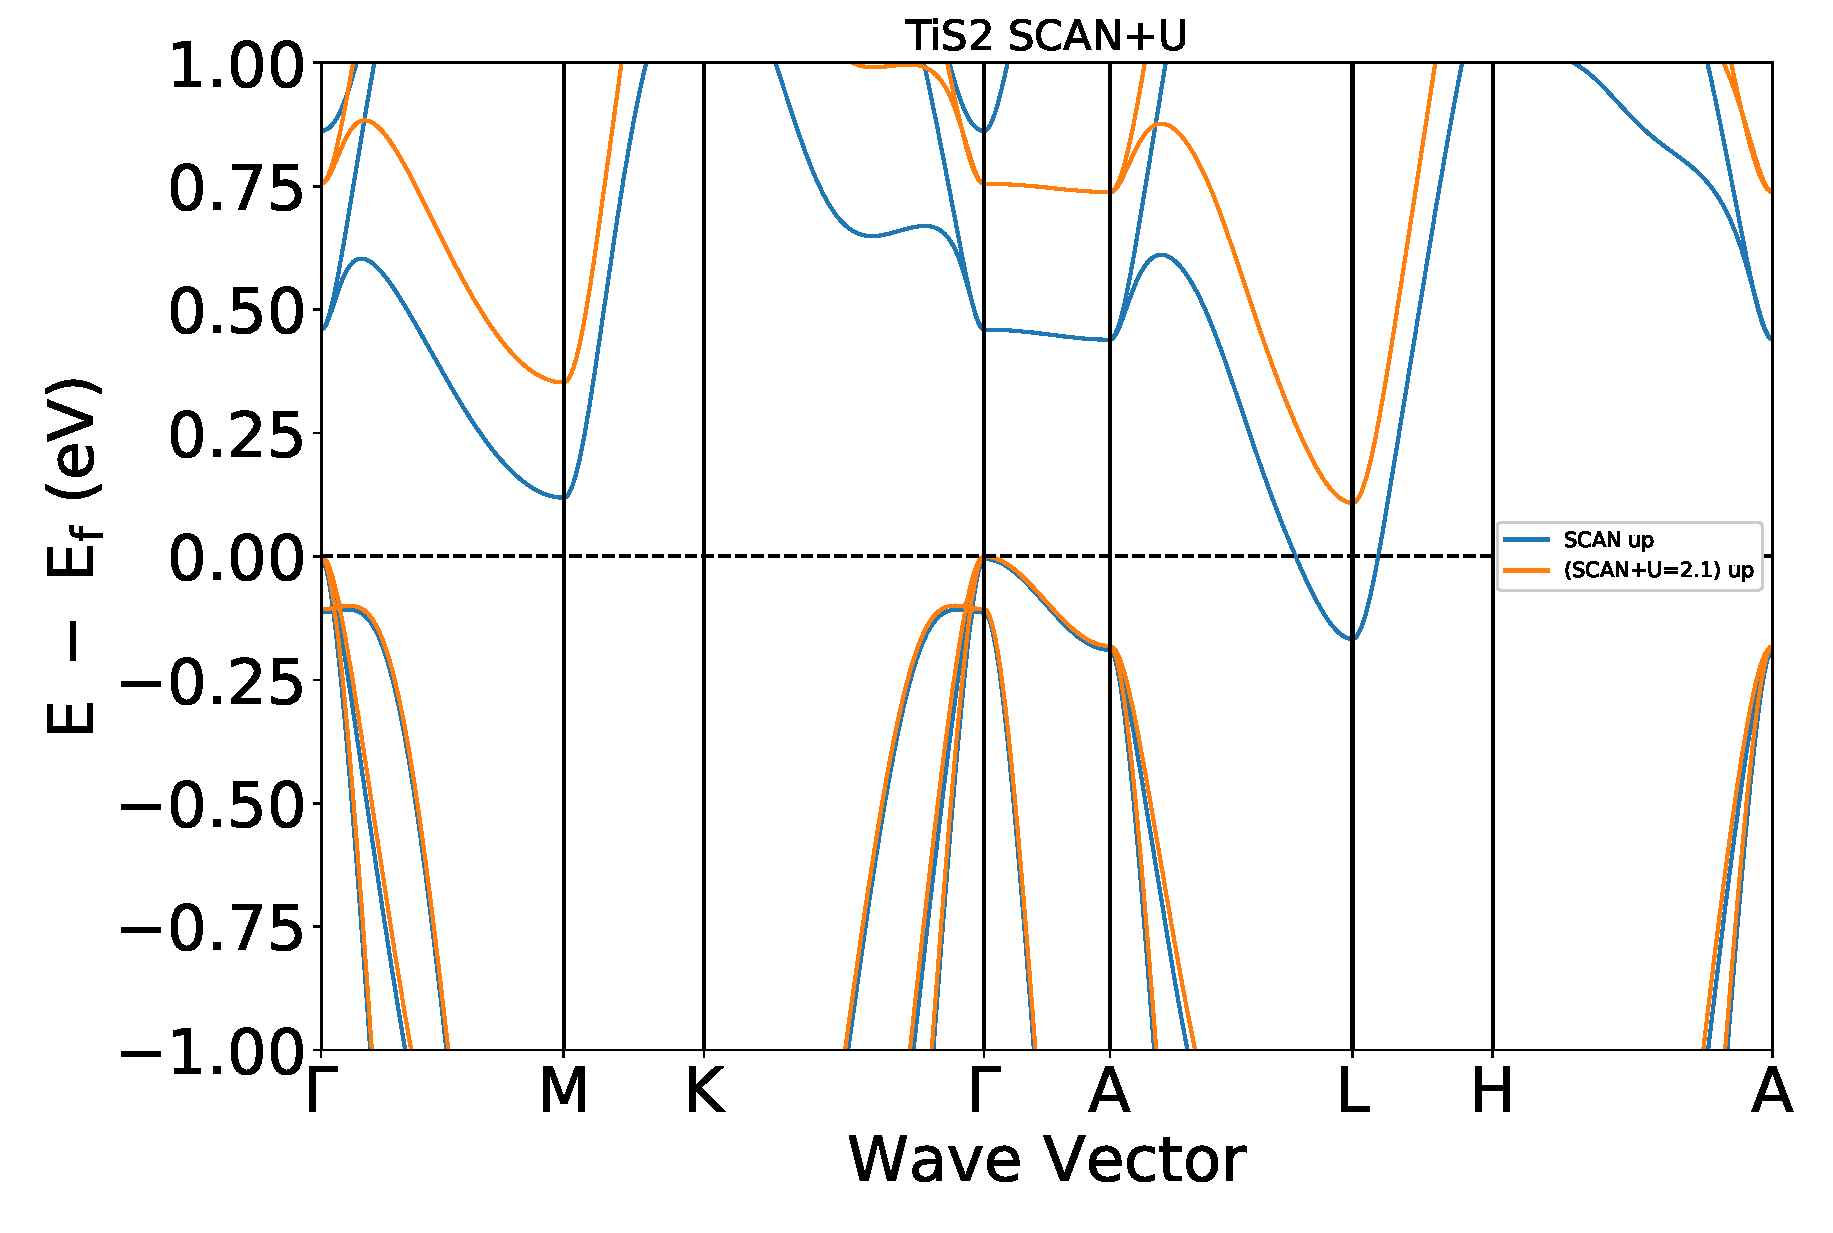
\includegraphics[scale=0.6]{results/TiS2_SCAN_vs._SCAN+U.eps}
	\caption{Електрона будова TiS$_2$ SCAN + U (U = 2.1)}\label{fig:SCAN+U_tis2}
\end{figure}

\begin{figure}
	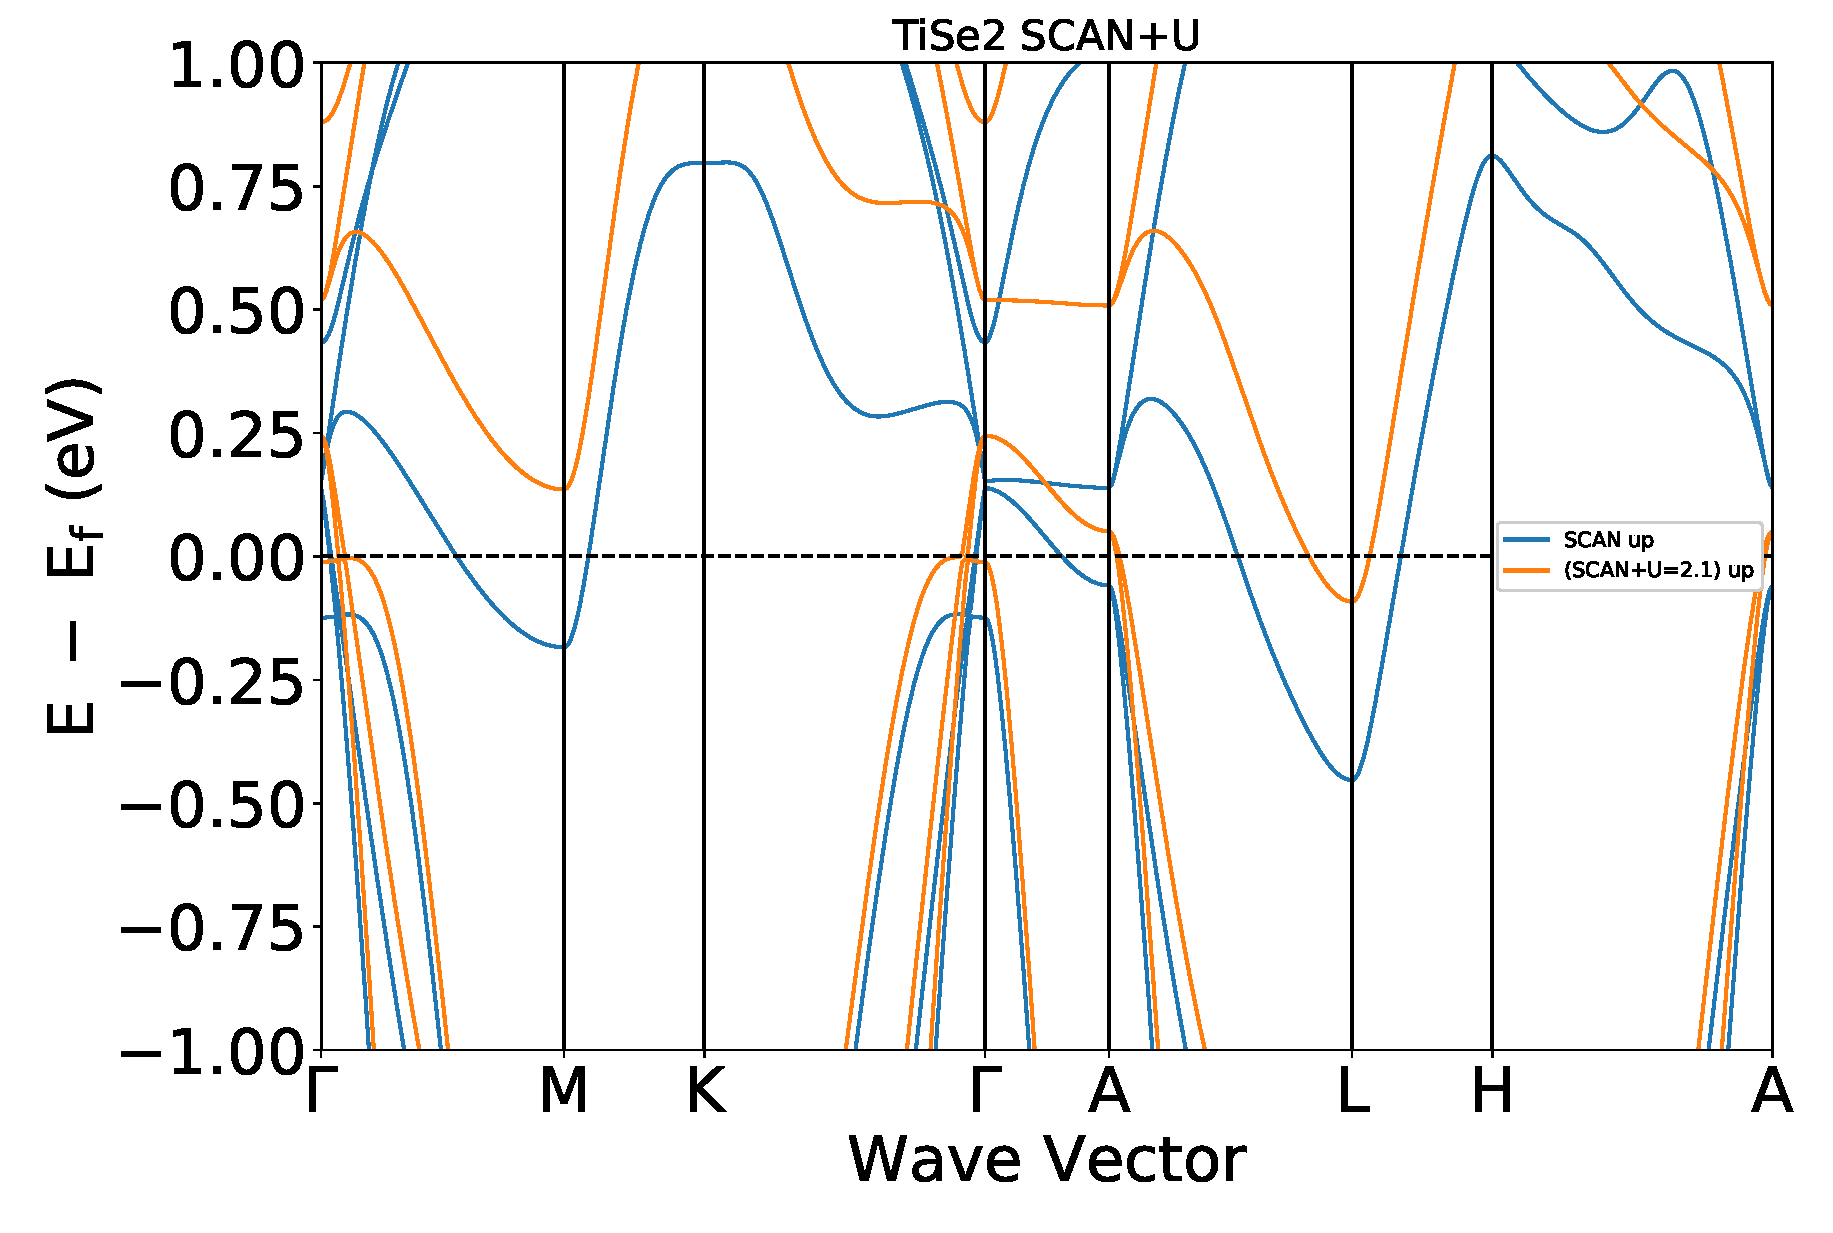
\includegraphics[scale=0.6]{results/TiSe2_SCAN_vs._SCAN+U.eps}
	\caption{Електрона будова TiSe$_2$ SCAN + U (U = 2.1)}\label{fig:SCAN+U_tise2}
\end{figure}

\begin{figure}
	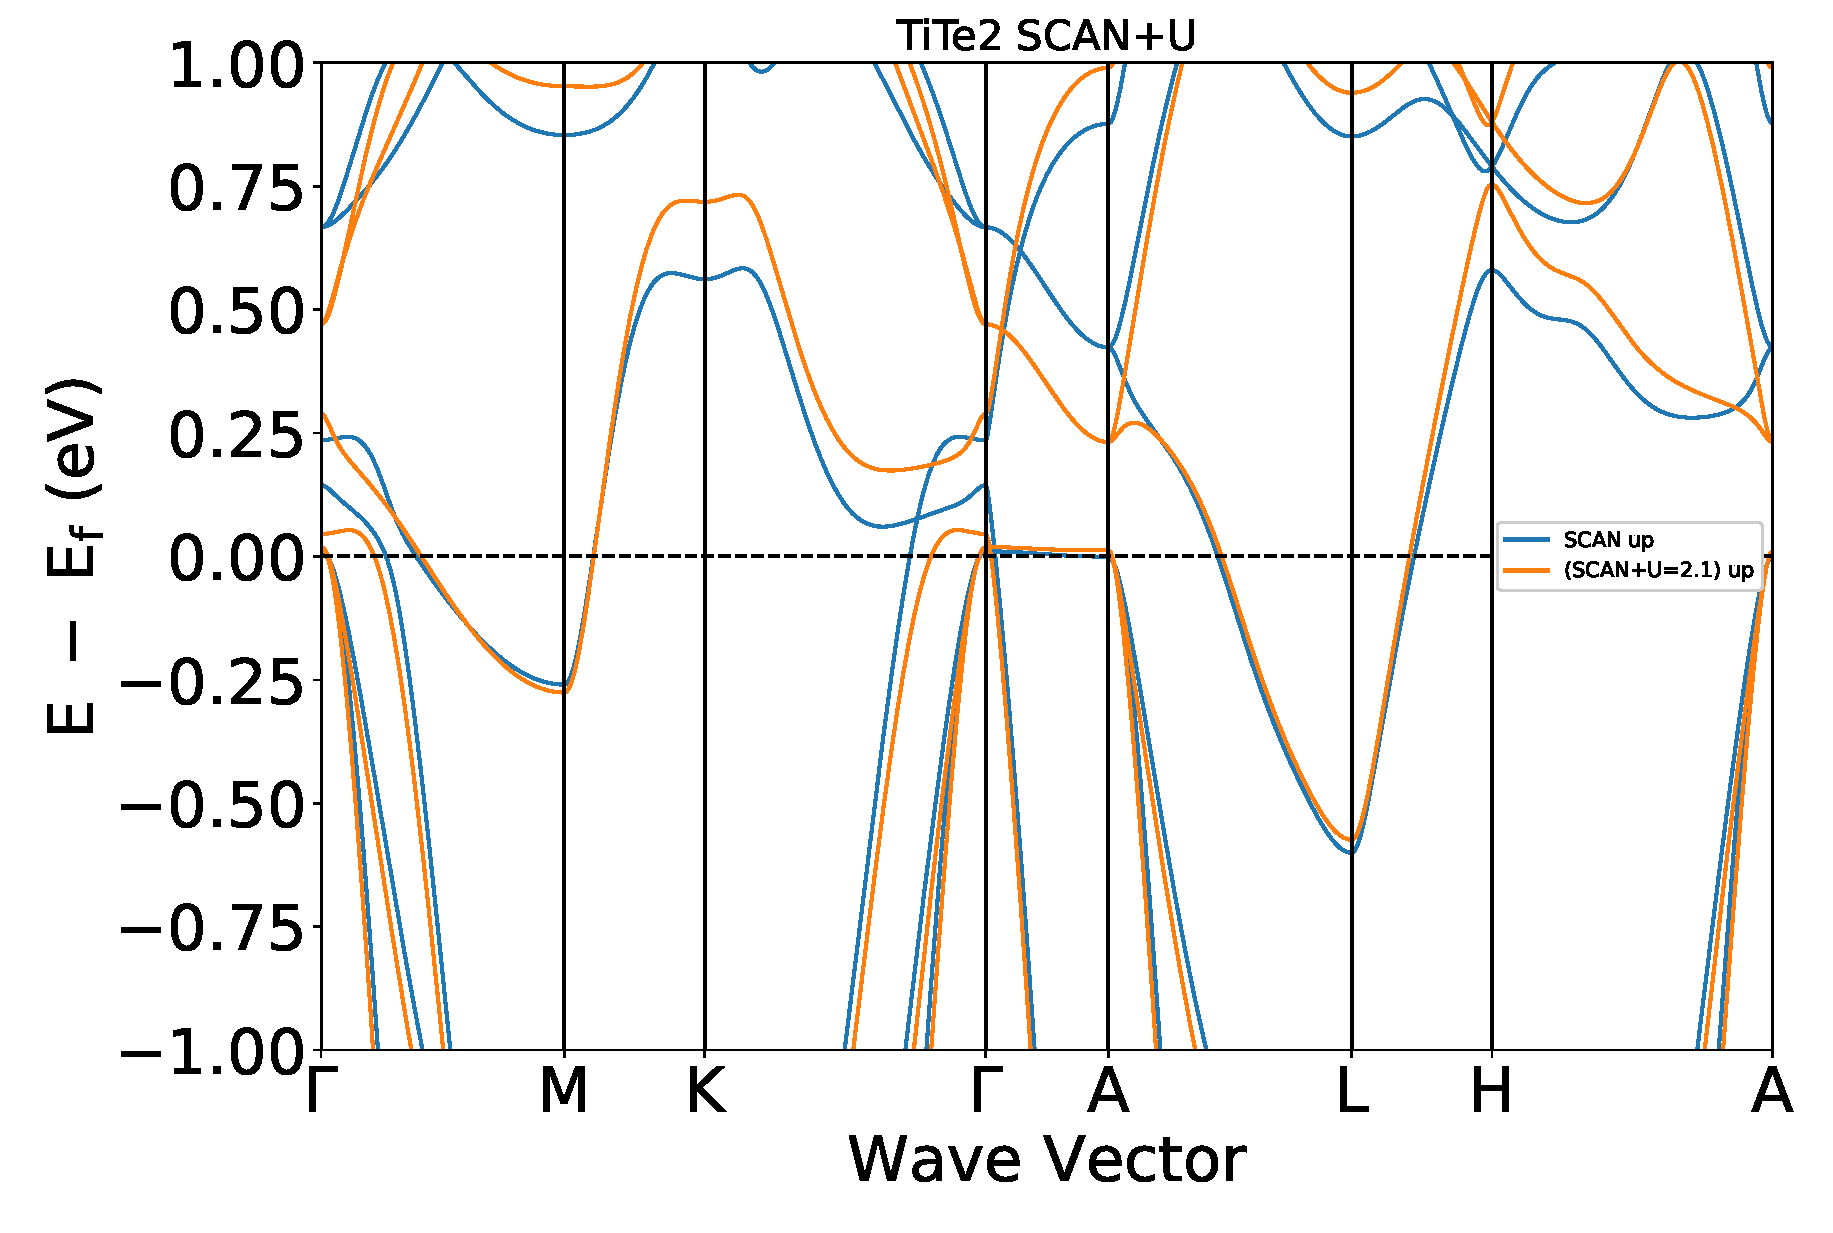
\includegraphics[scale=0.6]{results/TiTe2_SCAN_vs._SCAN+U.eps}
	\caption{Електрона будова TiTe$_2$ SCAN + U (U = 2.1)}\label{fig:SCAN+U_tite2}
\end{figure}

\section{Висновки до розділу}
У останньому розділі були представлені результати DFT розрахунків у SCAN наближені. Був проведений аналіз розрахунків, побудовані зони спектри та наведені таблиці постійних ґраток в порівнянні з PBE GGA функціоналом. Виявлені оптимальні значення параметра U, встановлено що U дорівнює 2.1 eV для відкриття енергетичної щілини. 
\addcontentsline{toc}{chapter}{Висновки}
\chapter*{Висновки}
Ми разрохували електроні властивості 1T-TiX$_2$ (X = S, Se, Te) і виявили що вони мають напівметалеву природу, окрім TiS$_2$. TiTe$_2$, TiSe$_2$ мають перекриття між смугами p і d халькогену та титану відповідно. DOS збільшується біля E$_F$ при переході від S до Te, Se, це може відбуватися із-за того, що перекриття Ti $d$ та Te, Se $p$ орбіталей у даних сполуках більше ніж з S, або як ми дослідили, воно зовсьм відсутнє і це добре узгоджується за нещодавними експериментами.

Для того щоб правильно описати щілину у TiS$_2$ знадобилось додаково взяти до уваги що це сильнокорельована система та до SCAN функціоналу додати взаємодію Хаббарда. Були установлені оптимальне значення U, яке складає 2.1 eV при якому щілина відкривається приблизно $\approx$ 0.1 eV. Потім було використано ван-дер-Ваальсову поправку rVV10 і ми змогли наблизитись до експериментальних значень щілини $\approx$ 0.22 eV. 
\addcontentsline{toc}{chapter}{Бібліоґрафія}
\bibliographystyle{unsrt}
\bibliography{biliog}
\end{document}
